\documentclass{report}


%%%%%%%%%%%%%%%%%%%%%%%%%%%%%%%%%
% PACKAGE IMPORTS
%%%%%%%%%%%%%%%%%%%%%%%%%%%%%%%%%


\usepackage[tmargin=2cm,rmargin=1in,lmargin=1in,margin=0.85in,bmargin=2cm,footskip=.2in,textwidth=12cm]{geometry}
\usepackage{amsmath,amsfonts,amsthm,amssymb,mathtools}
\usepackage[varbb]{newpxmath}
\usepackage{xfrac}
\usepackage[makeroom]{cancel}
\usepackage{mathtools}
\usepackage{bookmark}
\usepackage{enumitem}
\usepackage{hyperref,theoremref}
\usepackage{graphicx}
\usepackage{subfigure}

\hypersetup{
	pdftitle={Assignment},
	colorlinks=true, linkcolor=doc!90,
	bookmarksnumbered=true,
	bookmarksopen=true
}
\usepackage[most,many,breakable]{tcolorbox}
\usepackage{xcolor}
\usepackage{varwidth}
\usepackage{varwidth}
\usepackage{etoolbox}
%\usepackage{authblk}
\usepackage{nameref}
\usepackage{multicol,array}
\usepackage{tikz-cd}
\usepackage[ruled,vlined,linesnumbered]{algorithm2e}
\usepackage{comment} % enables the use of multi-line comments (\ifx \fi) 
\usepackage{import}
\usepackage{xifthen}
\usepackage{pdfpages}
\usepackage{transparent}
\usepackage{parskip}
\usepackage{blindtext}
\usepackage{booktabs}
\usepackage{listings}
\usepackage{multirow}
% \usepackage[paperheight=16cm,paperwidth=14cm,textwidth=12cm]{geometry}

\newcommand\mycommfont[1]{\footnotesize\ttfamily\textcolor{blue}{#1}}
\SetCommentSty{mycommfont}
\newcommand{\incfig}[1]{%
    \def\svgwidth{\columnwidth}
    \import{./figures/}{#1.pdf_tex}
}

\usepackage{tikzsymbols}
\renewcommand\qedsymbol{$\Laughey$}


%\usepackage{import}
%\usepackage{xifthen}
%\usepackage{pdfpages}
%\usepackage{transparent}


%%%%%%%%%%%%%%%%%%%%%%%%%%%%%%
% SELF MADE COLORS
%%%%%%%%%%%%%%%%%%%%%%%%%%%%%%



\definecolor{myg}{RGB}{56, 140, 70}
\definecolor{myb}{RGB}{45, 111, 177}
\definecolor{myr}{RGB}{199, 68, 64}
\definecolor{mytheorembg}{HTML}{F2F2F9}
\definecolor{mytheoremfr}{HTML}{00007B}
\definecolor{mylenmabg}{HTML}{FFFAF8}
\definecolor{mylenmafr}{HTML}{983b0f}
\definecolor{mypropbg}{HTML}{f2fbfc}
\definecolor{mypropfr}{HTML}{191971}
\definecolor{myexamplebg}{HTML}{F2FBF8}
\definecolor{myexamplefr}{HTML}{88D6D1}
\definecolor{myexampleti}{HTML}{2A7F7F}
\definecolor{mydefinitbg}{HTML}{E5E5FF}
\definecolor{mydefinitfr}{HTML}{3F3FA3}
\definecolor{notesgreen}{RGB}{0,162,0}
\definecolor{myp}{RGB}{197, 92, 212}
\definecolor{mygr}{HTML}{2C3338}
\definecolor{myred}{RGB}{127,0,0}
\definecolor{myyellow}{RGB}{169,121,69}
\definecolor{myexercisebg}{HTML}{F2FBF8}
\definecolor{myexercisefg}{HTML}{88D6D1}


%%%%%%%%%%%%%%%%%%%%%%%%%%%%
% TCOLORBOX SETUPS
%%%%%%%%%%%%%%%%%%%%%%%%%%%%

\setlength{\parindent}{1cm}
%================================
% THEOREM BOX
%================================

\tcbuselibrary{theorems,skins,hooks}
\newtcbtheorem[number within=section]{Theorem}{Theorem}
{%
	enhanced,
	breakable,
	colback = mytheorembg,
	frame hidden,
	boxrule = 0sp,
	borderline west = {2pt}{0pt}{mytheoremfr},
	sharp corners,
	detach title,
	before upper = \tcbtitle\par\smallskip,
	coltitle = mytheoremfr,
	fonttitle = \bfseries\sffamily,
	description font = \mdseries,
	separator sign none,
	segmentation style={solid, mytheoremfr},
}
{th}

\tcbuselibrary{theorems,skins,hooks}
\newtcbtheorem[number within=chapter]{theorem}{Theorem}
{%
	enhanced,
	breakable,
	colback = mytheorembg,
	frame hidden,
	boxrule = 0sp,
	borderline west = {2pt}{0pt}{mytheoremfr},
	sharp corners,
	detach title,
	before upper = \tcbtitle\par\smallskip,
	coltitle = mytheoremfr,
	fonttitle = \bfseries\sffamily,
	description font = \mdseries,
	separator sign none,
	segmentation style={solid, mytheoremfr},
}
{th}


\tcbuselibrary{theorems,skins,hooks}
\newtcolorbox{Theoremcon}
{%
	enhanced
	,breakable
	,colback = mytheorembg
	,frame hidden
	,boxrule = 0sp
	,borderline west = {2pt}{0pt}{mytheoremfr}
	,sharp corners
	,description font = \mdseries
	,separator sign none
}

%================================
% Corollery
%================================
\tcbuselibrary{theorems,skins,hooks}
\newtcbtheorem[number within=section]{Corollary}{Corollary}
{%
	enhanced
	,breakable
	,colback = myp!10
	,frame hidden
	,boxrule = 0sp
	,borderline west = {2pt}{0pt}{myp!85!black}
	,sharp corners
	,detach title
	,before upper = \tcbtitle\par\smallskip
	,coltitle = myp!85!black
	,fonttitle = \bfseries\sffamily
	,description font = \mdseries
	,separator sign none
	,segmentation style={solid, myp!85!black}
}
{th}
\tcbuselibrary{theorems,skins,hooks}
\newtcbtheorem[number within=chapter]{corollary}{Corollary}
{%
	enhanced
	,breakable
	,colback = myp!10
	,frame hidden
	,boxrule = 0sp
	,borderline west = {2pt}{0pt}{myp!85!black}
	,sharp corners
	,detach title
	,before upper = \tcbtitle\par\smallskip
	,coltitle = myp!85!black
	,fonttitle = \bfseries\sffamily
	,description font = \mdseries
	,separator sign none
	,segmentation style={solid, myp!85!black}
}
{th}


%================================
% LENMA
%================================

\tcbuselibrary{theorems,skins,hooks}
\newtcbtheorem[number within=section]{Lenma}{Lenma}
{%
	enhanced,
	breakable,
	colback = mylenmabg,
	frame hidden,
	boxrule = 0sp,
	borderline west = {2pt}{0pt}{mylenmafr},
	sharp corners,
	detach title,
	before upper = \tcbtitle\par\smallskip,
	coltitle = mylenmafr,
	fonttitle = \bfseries\sffamily,
	description font = \mdseries,
	separator sign none,
	segmentation style={solid, mylenmafr},
}
{th}

\tcbuselibrary{theorems,skins,hooks}
\newtcbtheorem[number within=chapter]{lenma}{Lenma}
{%
	enhanced,
	breakable,
	colback = mylenmabg,
	frame hidden,
	boxrule = 0sp,
	borderline west = {2pt}{0pt}{mylenmafr},
	sharp corners,
	detach title,
	before upper = \tcbtitle\par\smallskip,
	coltitle = mylenmafr,
	fonttitle = \bfseries\sffamily,
	description font = \mdseries,
	separator sign none,
	segmentation style={solid, mylenmafr},
}
{th}


%================================
% PROPOSITION
%================================

\tcbuselibrary{theorems,skins,hooks}
\newtcbtheorem[number within=section]{Prop}{Proposition}
{%
	enhanced,
	breakable,
	colback = mypropbg,
	frame hidden,
	boxrule = 0sp,
	borderline west = {2pt}{0pt}{mypropfr},
	sharp corners,
	detach title,
	before upper = \tcbtitle\par\smallskip,
	coltitle = mypropfr,
	fonttitle = \bfseries\sffamily,
	description font = \mdseries,
	separator sign none,
	segmentation style={solid, mypropfr},
}
{th}

\tcbuselibrary{theorems,skins,hooks}
\newtcbtheorem[number within=chapter]{prop}{Proposition}
{%
	enhanced,
	breakable,
	colback = mypropbg,
	frame hidden,
	boxrule = 0sp,
	borderline west = {2pt}{0pt}{mypropfr},
	sharp corners,
	detach title,
	before upper = \tcbtitle\par\smallskip,
	coltitle = mypropfr,
	fonttitle = \bfseries\sffamily,
	description font = \mdseries,
	separator sign none,
	segmentation style={solid, mypropfr},
}
{th}

\lstset{
    language=Python,
    basicstyle=\ttfamily\small,
    keywordstyle=\color{blue},
    commentstyle=\color{green},
    numbers=left,
    numberstyle=\tiny\color{gray},
    frame=single,
    breaklines=true
}

%================================
% CLAIM
%================================

\tcbuselibrary{theorems,skins,hooks}
\newtcbtheorem[number within=section]{claim}{Claim}
{%
	enhanced
	,breakable
	,colback = myg!10
	,frame hidden
	,boxrule = 0sp
	,borderline west = {2pt}{0pt}{myg}
	,sharp corners
	,detach title
	,before upper = \tcbtitle\par\smallskip
	,coltitle = myg!85!black
	,fonttitle = \bfseries\sffamily
	,description font = \mdseries
	,separator sign none
	,segmentation style={solid, myg!85!black}
}
{th}



%================================
% Exercise
%================================

\tcbuselibrary{theorems,skins,hooks}
\newtcbtheorem[number within=section]{Exercise}{Exercise}
{%
	enhanced,
	breakable,
	colback = myexercisebg,
	frame hidden,
	boxrule = 0sp,
	borderline west = {2pt}{0pt}{myexercisefg},
	sharp corners,
	detach title,
	before upper = \tcbtitle\par\smallskip,
	coltitle = myexercisefg,
	fonttitle = \bfseries\sffamily,
	description font = \mdseries,
	separator sign none,
	segmentation style={solid, myexercisefg},
}
{th}

\tcbuselibrary{theorems,skins,hooks}
\newtcbtheorem[number within=chapter]{exercise}{Exercise}
{%
	enhanced,
	breakable,
	colback = myexercisebg,
	frame hidden,
	boxrule = 0sp,
	borderline west = {2pt}{0pt}{myexercisefg},
	sharp corners,
	detach title,
	before upper = \tcbtitle\par\smallskip,
	coltitle = myexercisefg,
	fonttitle = \bfseries\sffamily,
	description font = \mdseries,
	separator sign none,
	segmentation style={solid, myexercisefg},
}
{th}

%================================
% EXAMPLE BOX
%================================

\newtcbtheorem[number within=section]{Example}{Example}
{%
	colback = myexamplebg
	,breakable
	,colframe = myexamplefr
	,coltitle = myexampleti
	,boxrule = 1pt
	,sharp corners
	,detach title
	,before upper=\tcbtitle\par\smallskip
	,fonttitle = \bfseries
	,description font = \mdseries
	,separator sign none
	,description delimiters parenthesis
}
{ex}

\newtcbtheorem[number within=chapter]{example}{Example}
{%
	colback = myexamplebg
	,breakable
	,colframe = myexamplefr
	,coltitle = myexampleti
	,boxrule = 1pt
	,sharp corners
	,detach title
	,before upper=\tcbtitle\par\smallskip
	,fonttitle = \bfseries
	,description font = \mdseries
	,separator sign none
	,description delimiters parenthesis
}
{ex}

%================================
% DEFINITION BOX
%================================

\newtcbtheorem[number within=section]{Definition}{Definition}{enhanced,
	before skip=2mm,after skip=2mm, colback=red!5,colframe=red!80!black,boxrule=0.5mm,
	attach boxed title to top left={xshift=1cm,yshift*=1mm-\tcboxedtitleheight}, varwidth boxed title*=-3cm,
	boxed title style={frame code={
					\path[fill=tcbcolback]
					([yshift=-1mm,xshift=-1mm]frame.north west)
					arc[start angle=0,end angle=180,radius=1mm]
					([yshift=-1mm,xshift=1mm]frame.north east)
					arc[start angle=180,end angle=0,radius=1mm];
					\path[left color=tcbcolback!60!black,right color=tcbcolback!60!black,
						middle color=tcbcolback!80!black]
					([xshift=-2mm]frame.north west) -- ([xshift=2mm]frame.north east)
					[rounded corners=1mm]-- ([xshift=1mm,yshift=-1mm]frame.north east)
					-- (frame.south east) -- (frame.south west)
					-- ([xshift=-1mm,yshift=-1mm]frame.north west)
					[sharp corners]-- cycle;
				},interior engine=empty,
		},
	fonttitle=\bfseries,
	title={#2},#1}{def}
\newtcbtheorem[number within=chapter]{definition}{Definition}{enhanced,
	before skip=2mm,after skip=2mm, colback=red!5,colframe=red!80!black,boxrule=0.5mm,
	attach boxed title to top left={xshift=1cm,yshift*=1mm-\tcboxedtitleheight}, varwidth boxed title*=-3cm,
	boxed title style={frame code={
					\path[fill=tcbcolback]
					([yshift=-1mm,xshift=-1mm]frame.north west)
					arc[start angle=0,end angle=180,radius=1mm]
					([yshift=-1mm,xshift=1mm]frame.north east)
					arc[start angle=180,end angle=0,radius=1mm];
					\path[left color=tcbcolback!60!black,right color=tcbcolback!60!black,
						middle color=tcbcolback!80!black]
					([xshift=-2mm]frame.north west) -- ([xshift=2mm]frame.north east)
					[rounded corners=1mm]-- ([xshift=1mm,yshift=-1mm]frame.north east)
					-- (frame.south east) -- (frame.south west)
					-- ([xshift=-1mm,yshift=-1mm]frame.north west)
					[sharp corners]-- cycle;
				},interior engine=empty,
		},
	fonttitle=\bfseries,
	title={#2},#1}{def}



%================================
% Solution BOX
%================================

\makeatletter
\newtcbtheorem{question}{Question}{enhanced,
	breakable,
	colback=white,
	colframe=myb!80!black,
	attach boxed title to top left={yshift*=-\tcboxedtitleheight},
	fonttitle=\bfseries,
	title={#2},
	boxed title size=title,
	boxed title style={%
			sharp corners,
			rounded corners=northwest,
			colback=tcbcolframe,
			boxrule=0pt,
		},
	underlay boxed title={%
			\path[fill=tcbcolframe] (title.south west)--(title.south east)
			to[out=0, in=180] ([xshift=5mm]title.east)--
			(title.center-|frame.east)
			[rounded corners=\kvtcb@arc] |-
			(frame.north) -| cycle;
		},
	#1
}{def}
\makeatother

%================================
% SOLUTION BOX
%================================

\makeatletter
\newtcolorbox{solution}{enhanced,
	breakable,
	colback=white,
	colframe=myg!80!black,
	attach boxed title to top left={yshift*=-\tcboxedtitleheight},
	title=Solution,
	boxed title size=title,
	boxed title style={%
			sharp corners,
			rounded corners=northwest,
			colback=tcbcolframe,
			boxrule=0pt,
		},
	underlay boxed title={%
			\path[fill=tcbcolframe] (title.south west)--(title.south east)
			to[out=0, in=180] ([xshift=5mm]title.east)--
			(title.center-|frame.east)
			[rounded corners=\kvtcb@arc] |-
			(frame.north) -| cycle;
		},
}
\makeatother

%================================
% Question BOX
%================================

\makeatletter
\newtcbtheorem{qstion}{Question}{enhanced,
	breakable,
	colback=white,
	colframe=mygr,
	attach boxed title to top left={yshift*=-\tcboxedtitleheight},
	fonttitle=\bfseries,
	title={#2},
	boxed title size=title,
	boxed title style={%
			sharp corners,
			rounded corners=northwest,
			colback=tcbcolframe,
			boxrule=0pt,
		},
	underlay boxed title={%
			\path[fill=tcbcolframe] (title.south west)--(title.south east)
			to[out=0, in=180] ([xshift=5mm]title.east)--
			(title.center-|frame.east)
			[rounded corners=\kvtcb@arc] |-
			(frame.north) -| cycle;
		},
	#1
}{def}
\makeatother

\newtcbtheorem[number within=chapter]{wconc}{Wrong Concept}{
	breakable,
	enhanced,
	colback=white,
	colframe=myr,
	arc=0pt,
	outer arc=0pt,
	fonttitle=\bfseries\sffamily\large,
	colbacktitle=myr,
	attach boxed title to top left={},
	boxed title style={
			enhanced,
			skin=enhancedfirst jigsaw,
			arc=3pt,
			bottom=0pt,
			interior style={fill=myr}
		},
	#1
}{def}



%================================
% NOTE BOX
%================================

\usetikzlibrary{arrows,calc,shadows.blur}
\tcbuselibrary{skins}
\newtcolorbox{note}[1][]{%
	enhanced jigsaw,
	colback=gray!20!white,%
	colframe=gray!80!black,
	size=small,
	boxrule=1pt,
	title=\textbf{Note:-},
	halign title=flush center,
	coltitle=black,
	breakable,
	drop shadow=black!50!white,
	attach boxed title to top left={xshift=1cm,yshift=-\tcboxedtitleheight/2,yshifttext=-\tcboxedtitleheight/2},
	minipage boxed title=1.5cm,
	boxed title style={%
			colback=white,
			size=fbox,
			boxrule=1pt,
			boxsep=2pt,
			underlay={%
					\coordinate (dotA) at ($(interior.west) + (-0.5pt,0)$);
					\coordinate (dotB) at ($(interior.east) + (0.5pt,0)$);
					\begin{scope}
						\clip (interior.north west) rectangle ([xshift=3ex]interior.east);
						\filldraw [white, blur shadow={shadow opacity=60, shadow yshift=-.75ex}, rounded corners=2pt] (interior.north west) rectangle (interior.south east);
					\end{scope}
					\begin{scope}[gray!80!black]
						\fill (dotA) circle (2pt);
						\fill (dotB) circle (2pt);
					\end{scope}
				},
		},
	#1,
}

%%%%%%%%%%%%%%%%%%%%%%%%%%%%%%
% SELF MADE COMMANDS
%%%%%%%%%%%%%%%%%%%%%%%%%%%%%%


\newcommand{\thm}[2]{\begin{Theorem}{#1}{}#2\end{Theorem}}
\newcommand{\cor}[2]{\begin{Corollary}{#1}{}#2\end{Corollary}}
\newcommand{\mlenma}[2]{\begin{Lenma}{#1}{}#2\end{Lenma}}
\newcommand{\mprop}[2]{\begin{Prop}{#1}{}#2\end{Prop}}
\newcommand{\clm}[3]{\begin{claim}{#1}{#2}#3\end{claim}}
\newcommand{\wc}[2]{\begin{wconc}{#1}{}\setlength{\parindent}{1cm}#2\end{wconc}}
\newcommand{\thmcon}[1]{\begin{Theoremcon}{#1}\end{Theoremcon}}
\newcommand{\ex}[2]{\begin{Example}{#1}{}#2\end{Example}}
\newcommand{\dfn}[2]{\begin{Definition}[colbacktitle=red!75!black]{#1}{}#2\end{Definition}}
\newcommand{\dfnc}[2]{\begin{definition}[colbacktitle=red!75!black]{#1}{}#2\end{definition}}
\newcommand{\qs}[2]{\begin{question}{#1}{}#2\end{question}}
\newcommand{\pf}[2]{\begin{myproof}[#1]#2\end{myproof}}
\newcommand{\nt}[1]{\begin{note}#1\end{note}}

\newcommand*\circled[1]{\tikz[baseline=(char.base)]{
		\node[shape=circle,draw,inner sep=1pt] (char) {#1};}}
\newcommand\getcurrentref[1]{%
	\ifnumequal{\value{#1}}{0}
	{??}
	{\the\value{#1}}%
}
\newcommand{\getCurrentSectionNumber}{\getcurrentref{section}}
\newenvironment{myproof}[1][\proofname]{%
	\proof[\bfseries #1: ]%
}{\endproof}

\newcommand{\mclm}[2]{\begin{myclaim}[#1]#2\end{myclaim}}
\newenvironment{myclaim}[1][\claimname]{\proof[\bfseries #1: ]}{}

\newcounter{mylabelcounter}

\makeatletter
\newcommand{\setword}[2]{%
	\phantomsection
	#1\def\@currentlabel{\unexpanded{#1}}\label{#2}%
}
\makeatother




\tikzset{
	symbol/.style={
			draw=none,
			every to/.append style={
					edge node={node [sloped, allow upside down, auto=false]{$#1$}}}
		}
}


% deliminators
\DeclarePairedDelimiter{\abs}{\lvert}{\rvert}
\DeclarePairedDelimiter{\norm}{\lVert}{\rVert}

\DeclarePairedDelimiter{\ceil}{\lceil}{\rceil}
\DeclarePairedDelimiter{\floor}{\lfloor}{\rfloor}
\DeclarePairedDelimiter{\round}{\lfloor}{\rceil}

\newsavebox\diffdbox
\newcommand{\slantedromand}{{\mathpalette\makesl{d}}}
\newcommand{\makesl}[2]{%
\begingroup
\sbox{\diffdbox}{$\mathsurround=0pt#1\mathrm{#2}$}%
\pdfsave
\pdfsetmatrix{1 0 0.2 1}%
\rlap{\usebox{\diffdbox}}%
\pdfrestore
\hskip\wd\diffdbox
\endgroup
}
\newcommand{\dd}[1][]{\ensuremath{\mathop{}\!\ifstrempty{#1}{%
\slantedromand\@ifnextchar^{\hspace{0.2ex}}{\hspace{0.1ex}}}%
{\slantedromand\hspace{0.2ex}^{#1}}}}
\ProvideDocumentCommand\dv{o m g}{%
  \ensuremath{%
    \IfValueTF{#3}{%
      \IfNoValueTF{#1}{%
        \frac{\dd #2}{\dd #3}%
      }{%
        \frac{\dd^{#1} #2}{\dd #3^{#1}}%
      }%
    }{%
      \IfNoValueTF{#1}{%
        \frac{\dd}{\dd #2}%
      }{%
        \frac{\dd^{#1}}{\dd #2^{#1}}%
      }%
    }%
  }%
}
\providecommand*{\pdv}[3][]{\frac{\partial^{#1}#2}{\partial#3^{#1}}}
%  - others
\DeclareMathOperator{\Lap}{\mathcal{L}}
\DeclareMathOperator{\Var}{Var} % varience
\DeclareMathOperator{\Cov}{Cov} % covarience
\DeclareMathOperator{\E}{E} % expected

% Since the amsthm package isn't loaded

% I prefer the slanted \leq
\let\oldleq\leq % save them in case they're every wanted
\let\oldgeq\geq
\renewcommand{\leq}{\leqslant}
\renewcommand{\geq}{\geqslant}




%%%%%%%%%%%%%%%%%%%%%%%%%%%%%%%%%%%%%%%%%%%
% TABLE OF CONTENTS
%%%%%%%%%%%%%%%%%%%%%%%%%%%%%%%%%%%%%%%%%%%

\usepackage{tikz}
\definecolor{doc}{RGB}{0,60,110}
\usepackage{titletoc}
\contentsmargin{0cm}
\titlecontents{chapter}[3.7pc]
{\addvspace{30pt}%
	\begin{tikzpicture}[remember picture, overlay]%
		\draw[fill=doc!60,draw=doc!60] (-7,-.1) rectangle (-0.9,.5);%
		\pgftext[left,x=-3.5cm,y=0.2cm]{\color{white}\Large\sc\bfseries Chapter\ \thecontentslabel};%
	\end{tikzpicture}\color{doc!60}\large\sc\bfseries}%
{}
{}
{\;\titlerule\;\large\sc\bfseries Page \thecontentspage
	\begin{tikzpicture}[remember picture, overlay]
		\draw[fill=doc!60,draw=doc!60] (2pt,0) rectangle (4,0.1pt);
	\end{tikzpicture}}%
\titlecontents{section}[3.7pc]
{\addvspace{2pt}}
{\contentslabel[\thecontentslabel]{2pc}}
{}
{\hfill\small \thecontentspage}
[]
\titlecontents*{subsection}[3.7pc]
{\addvspace{-1pt}\small}
{}
{}
{\ --- \small\thecontentspage}
[ \textbullet\ ][]

\makeatletter
\renewcommand{\tableofcontents}{%
	\chapter*{%
	  \vspace*{-20\p@}%
	  \begin{tikzpicture}[remember picture, overlay]%
		  \pgftext[right,x=15cm,y=0.2cm]{\color{doc!60}\Huge\sc\bfseries \contentsname};%
		  \draw[fill=doc!60,draw=doc!60] (13,-.75) rectangle (20,1);%
		  \clip (13,-.75) rectangle (20,1);
		  \pgftext[right,x=15cm,y=0.2cm]{\color{white}\Huge\sc\bfseries \contentsname};%
	  \end{tikzpicture}}%
	\@starttoc{toc}}
\makeatother


%From M275 "Topology" at SJSU
\newcommand{\id}{\mathrm{id}}
\newcommand{\taking}[1]{\xrightarrow{#1}}
\newcommand{\inv}{^{-1}}


\DeclareMathOperator{\diam}{diam}
\DeclareMathOperator{\ord}{ord}
\newcommand{\defeq}{\overset{\mathrm{def}}{=}}

%From the USAMO .tex files
\newcommand{\ts}{\textsuperscript}
\newcommand{\dg}{^\circ}
\newcommand{\ii}{\item}



\newcommand{\liff}{\leftrightarrow}
\newcommand{\lthen}{\rightarrow}
\newcommand{\opname}{\operatorname}
\newcommand{\surjto}{\twoheadrightarrow}
\newcommand{\injto}{\hookrightarrow}
\newcommand{\On}{\mathrm{On}} % ordinals
\DeclareMathOperator{\img}{im} % Image
\DeclareMathOperator{\Img}{Im} % Image
\DeclareMathOperator{\coker}{coker} % Cokernel
\DeclareMathOperator{\Coker}{Coker} % Cokernel
\DeclareMathOperator{\Ker}{Ker} % Kernel
\DeclareMathOperator{\rank}{rank}
\DeclareMathOperator{\Spec}{Spec} % spectrum
\DeclareMathOperator{\Tr}{Tr} % trace
\DeclareMathOperator{\pr}{pr} % projection
\DeclareMathOperator{\ext}{ext} % extension
\DeclareMathOperator{\pred}{pred} % predecessor
\DeclareMathOperator{\dom}{dom} % domain
\DeclareMathOperator{\ran}{ran} % range
\DeclareMathOperator{\Hom}{Hom} % homomorphism
\DeclareMathOperator{\Mor}{Mor} % morphisms
\DeclareMathOperator{\End}{End} % endomorphism

\newcommand{\eps}{\epsilon}
\newcommand{\veps}{\varepsilon}
\newcommand{\ol}{\overline}
\newcommand{\ul}{\underline}
\newcommand{\wt}{\widetilde}
\newcommand{\wh}{\widehat}
\newcommand{\vocab}[1]{\textbf{\color{blue} #1}}
\providecommand{\half}{\frac{1}{2}}
\newcommand{\dang}{\measuredangle} %% Directed angle
\newcommand{\ray}[1]{\overrightarrow{#1}}
\newcommand{\seg}[1]{\overline{#1}}
\newcommand{\arc}[1]{\wideparen{#1}}
\DeclareMathOperator{\cis}{cis}
\DeclareMathOperator*{\lcm}{lcm}
\DeclareMathOperator*{\argmin}{arg min}
\DeclareMathOperator*{\argmax}{arg max}
\newcommand{\cycsum}{\sum_{\mathrm{cyc}}}
\newcommand{\symsum}{\sum_{\mathrm{sym}}}
\newcommand{\cycprod}{\prod_{\mathrm{cyc}}}
\newcommand{\symprod}{\prod_{\mathrm{sym}}}
\newcommand{\Qed}{\begin{flushright}\qed\end{flushright}}
\newcommand{\parinn}{\setlength{\parindent}{1cm}}
\newcommand{\parinf}{\setlength{\parindent}{0cm}}
% \newcommand{\norm}{\|\cdot\|}
\newcommand{\inorm}{\norm_{\infty}}
\newcommand{\opensets}{\{V_{\alpha}\}_{\alpha\in I}}
\newcommand{\oset}{V_{\alpha}}
\newcommand{\opset}[1]{V_{\alpha_{#1}}}
\newcommand{\lub}{\text{lub}}
\newcommand{\del}[2]{\frac{\partial #1}{\partial #2}}
\newcommand{\Del}[3]{\frac{\partial^{#1} #2}{\partial^{#1} #3}}
\newcommand{\deld}[2]{\dfrac{\partial #1}{\partial #2}}
\newcommand{\Deld}[3]{\dfrac{\partial^{#1} #2}{\partial^{#1} #3}}
\newcommand{\lm}{\lambda}
\newcommand{\uin}{\mathbin{\rotatebox[origin=c]{90}{$\in$}}}
\newcommand{\usubset}{\mathbin{\rotatebox[origin=c]{90}{$\subset$}}}
\newcommand{\lt}{\left}
\newcommand{\rt}{\right}
\newcommand{\bs}[1]{\boldsymbol{#1}}
\newcommand{\exs}{\exists}
\newcommand{\st}{\strut}
\newcommand{\dps}[1]{\displaystyle{#1}}

\newcommand{\sol}{\setlength{\parindent}{0cm}\textbf{\textit{Solution:}}\setlength{\parindent}{1cm} }
\newcommand{\solve}[1]{\setlength{\parindent}{0cm}\textbf{\textit{Solution: }}\setlength{\parindent}{1cm}#1 \Qed}

% Things Lie
\newcommand{\kb}{\mathfrak b}
\newcommand{\kg}{\mathfrak g}
\newcommand{\kh}{\mathfrak h}
\newcommand{\kn}{\mathfrak n}
\newcommand{\ku}{\mathfrak u}
\newcommand{\kz}{\mathfrak z}
\DeclareMathOperator{\Ext}{Ext} % Ext functor
\DeclareMathOperator{\Tor}{Tor} % Tor functor
\newcommand{\gl}{\opname{\mathfrak{gl}}} % frak gl group
\renewcommand{\sl}{\opname{\mathfrak{sl}}} % frak sl group chktex 6

% More script letters etc.
\newcommand{\SA}{\mathcal A}
\newcommand{\SB}{\mathcal B}
\newcommand{\SC}{\mathcal C}
\newcommand{\SF}{\mathcal F}
\newcommand{\SG}{\mathcal G}
\newcommand{\SH}{\mathcal H}
\newcommand{\OO}{\mathcal O}

\newcommand{\SCA}{\mathscr A}
\newcommand{\SCB}{\mathscr B}
\newcommand{\SCC}{\mathscr C}
\newcommand{\SCD}{\mathscr D}
\newcommand{\SCE}{\mathscr E}
\newcommand{\SCF}{\mathscr F}
\newcommand{\SCG}{\mathscr G}
\newcommand{\SCH}{\mathscr H}

% Mathfrak primes
\newcommand{\km}{\mathfrak m}
\newcommand{\kp}{\mathfrak p}
\newcommand{\kq}{\mathfrak q}

% number sets
\newcommand{\RR}[1][]{\ensuremath{\ifstrempty{#1}{\mathbb{R}}{\mathbb{R}^{#1}}}}
\newcommand{\NN}[1][]{\ensuremath{\ifstrempty{#1}{\mathbb{N}}{\mathbb{N}^{#1}}}}
\newcommand{\ZZ}[1][]{\ensuremath{\ifstrempty{#1}{\mathbb{Z}}{\mathbb{Z}^{#1}}}}
\newcommand{\QQ}[1][]{\ensuremath{\ifstrempty{#1}{\mathbb{Q}}{\mathbb{Q}^{#1}}}}
\newcommand{\CC}[1][]{\ensuremath{\ifstrempty{#1}{\mathbb{C}}{\mathbb{C}^{#1}}}}
\newcommand{\PP}[1][]{\ensuremath{\ifstrempty{#1}{\mathbb{P}}{\mathbb{P}^{#1}}}}
\newcommand{\HH}[1][]{\ensuremath{\ifstrempty{#1}{\mathbb{H}}{\mathbb{H}^{#1}}}}
\newcommand{\FF}[1][]{\ensuremath{\ifstrempty{#1}{\mathbb{F}}{\mathbb{F}^{#1}}}}
% expected value
\newcommand{\EE}{\ensuremath{\mathbb{E}}}
\newcommand{\charin}{\text{ char }}
\DeclareMathOperator{\sign}{sign}
\DeclareMathOperator{\Aut}{Aut}
\DeclareMathOperator{\Inn}{Inn}
\DeclareMathOperator{\Syl}{Syl}
\DeclareMathOperator{\Gal}{Gal}
\DeclareMathOperator{\GL}{GL} % General linear group
\DeclareMathOperator{\SL}{SL} % Special linear group

%---------------------------------------
% BlackBoard Math Fonts :-
%---------------------------------------

%Captital Letters
\newcommand{\bbA}{\mathbb{A}}	\newcommand{\bbB}{\mathbb{B}}
\newcommand{\bbC}{\mathbb{C}}	\newcommand{\bbD}{\mathbb{D}}
\newcommand{\bbE}{\mathbb{E}}	\newcommand{\bbF}{\mathbb{F}}
\newcommand{\bbG}{\mathbb{G}}	\newcommand{\bbH}{\mathbb{H}}
\newcommand{\bbI}{\mathbb{I}}	\newcommand{\bbJ}{\mathbb{J}}
\newcommand{\bbK}{\mathbb{K}}	\newcommand{\bbL}{\mathbb{L}}
\newcommand{\bbM}{\mathbb{M}}	\newcommand{\bbN}{\mathbb{N}}
\newcommand{\bbO}{\mathbb{O}}	\newcommand{\bbP}{\mathbb{P}}
\newcommand{\bbQ}{\mathbb{Q}}	\newcommand{\bbR}{\mathbb{R}}
\newcommand{\bbS}{\mathbb{S}}	\newcommand{\bbT}{\mathbb{T}}
\newcommand{\bbU}{\mathbb{U}}	\newcommand{\bbV}{\mathbb{V}}
\newcommand{\bbW}{\mathbb{W}}	\newcommand{\bbX}{\mathbb{X}}
\newcommand{\bbY}{\mathbb{Y}}	\newcommand{\bbZ}{\mathbb{Z}}

%---------------------------------------
% MathCal Fonts :-
%---------------------------------------

%Captital Letters
\newcommand{\mcA}{\mathcal{A}}	\newcommand{\mcB}{\mathcal{B}}
\newcommand{\mcC}{\mathcal{C}}	\newcommand{\mcD}{\mathcal{D}}
\newcommand{\mcE}{\mathcal{E}}	\newcommand{\mcF}{\mathcal{F}}
\newcommand{\mcG}{\mathcal{G}}	\newcommand{\mcH}{\mathcal{H}}
\newcommand{\mcI}{\mathcal{I}}	\newcommand{\mcJ}{\mathcal{J}}
\newcommand{\mcK}{\mathcal{K}}	\newcommand{\mcL}{\mathcal{L}}
\newcommand{\mcM}{\mathcal{M}}	\newcommand{\mcN}{\mathcal{N}}
\newcommand{\mcO}{\mathcal{O}}	\newcommand{\mcP}{\mathcal{P}}
\newcommand{\mcQ}{\mathcal{Q}}	\newcommand{\mcR}{\mathcal{R}}
\newcommand{\mcS}{\mathcal{S}}	\newcommand{\mcT}{\mathcal{T}}
\newcommand{\mcU}{\mathcal{U}}	\newcommand{\mcV}{\mathcal{V}}
\newcommand{\mcW}{\mathcal{W}}	\newcommand{\mcX}{\mathcal{X}}
\newcommand{\mcY}{\mathcal{Y}}	\newcommand{\mcZ}{\mathcal{Z}}


%---------------------------------------
% Bold Math Fonts :-
%---------------------------------------

%Captital Letters
\newcommand{\bmA}{\boldsymbol{A}}	\newcommand{\bmB}{\boldsymbol{B}}
\newcommand{\bmC}{\boldsymbol{C}}	\newcommand{\bmD}{\boldsymbol{D}}
\newcommand{\bmE}{\boldsymbol{E}}	\newcommand{\bmF}{\boldsymbol{F}}
\newcommand{\bmG}{\boldsymbol{G}}	\newcommand{\bmH}{\boldsymbol{H}}
\newcommand{\bmI}{\boldsymbol{I}}	\newcommand{\bmJ}{\boldsymbol{J}}
\newcommand{\bmK}{\boldsymbol{K}}	\newcommand{\bmL}{\boldsymbol{L}}
\newcommand{\bmM}{\boldsymbol{M}}	\newcommand{\bmN}{\boldsymbol{N}}
\newcommand{\bmO}{\boldsymbol{O}}	\newcommand{\bmP}{\boldsymbol{P}}
\newcommand{\bmQ}{\boldsymbol{Q}}	\newcommand{\bmR}{\boldsymbol{R}}
\newcommand{\bmS}{\boldsymbol{S}}	\newcommand{\bmT}{\boldsymbol{T}}
\newcommand{\bmU}{\boldsymbol{U}}	\newcommand{\bmV}{\boldsymbol{V}}
\newcommand{\bmW}{\boldsymbol{W}}	\newcommand{\bmX}{\boldsymbol{X}}
\newcommand{\bmY}{\boldsymbol{Y}}	\newcommand{\bmZ}{\boldsymbol{Z}}
%Small Letters
\newcommand{\bma}{\boldsymbol{a}}	\newcommand{\bmb}{\boldsymbol{b}}
\newcommand{\bmc}{\boldsymbol{c}}	\newcommand{\bmd}{\boldsymbol{d}}
\newcommand{\bme}{\boldsymbol{e}}	\newcommand{\bmf}{\boldsymbol{f}}
\newcommand{\bmg}{\boldsymbol{g}}	\newcommand{\bmh}{\boldsymbol{h}}
\newcommand{\bmi}{\boldsymbol{i}}	\newcommand{\bmj}{\boldsymbol{j}}
\newcommand{\bmk}{\boldsymbol{k}}	\newcommand{\bml}{\boldsymbol{l}}
\newcommand{\bmm}{\boldsymbol{m}}	\newcommand{\bmn}{\boldsymbol{n}}
\newcommand{\bmo}{\boldsymbol{o}}	\newcommand{\bmp}{\boldsymbol{p}}
\newcommand{\bmq}{\boldsymbol{q}}	\newcommand{\bmr}{\boldsymbol{r}}
\newcommand{\bms}{\boldsymbol{s}}	\newcommand{\bmt}{\boldsymbol{t}}
\newcommand{\bmu}{\boldsymbol{u}}	\newcommand{\bmv}{\boldsymbol{v}}
\newcommand{\bmw}{\boldsymbol{w}}	\newcommand{\bmx}{\boldsymbol{x}}
\newcommand{\bmy}{\boldsymbol{y}}	\newcommand{\bmz}{\boldsymbol{z}}

%---------------------------------------
% Scr Math Fonts :-
%---------------------------------------

\newcommand{\sA}{{\mathscr{A}}}   \newcommand{\sB}{{\mathscr{B}}}
\newcommand{\sC}{{\mathscr{C}}}   \newcommand{\sD}{{\mathscr{D}}}
\newcommand{\sE}{{\mathscr{E}}}   \newcommand{\sF}{{\mathscr{F}}}
\newcommand{\sG}{{\mathscr{G}}}   \newcommand{\sH}{{\mathscr{H}}}
\newcommand{\sI}{{\mathscr{I}}}   \newcommand{\sJ}{{\mathscr{J}}}
\newcommand{\sK}{{\mathscr{K}}}   \newcommand{\sL}{{\mathscr{L}}}
\newcommand{\sM}{{\mathscr{M}}}   \newcommand{\sN}{{\mathscr{N}}}
\newcommand{\sO}{{\mathscr{O}}}   \newcommand{\sP}{{\mathscr{P}}}
\newcommand{\sQ}{{\mathscr{Q}}}   \newcommand{\sR}{{\mathscr{R}}}
\newcommand{\sS}{{\mathscr{S}}}   \newcommand{\sT}{{\mathscr{T}}}
\newcommand{\sU}{{\mathscr{U}}}   \newcommand{\sV}{{\mathscr{V}}}
\newcommand{\sW}{{\mathscr{W}}}   \newcommand{\sX}{{\mathscr{X}}}
\newcommand{\sY}{{\mathscr{Y}}}   \newcommand{\sZ}{{\mathscr{Z}}}


%---------------------------------------
% Math Fraktur Font
%---------------------------------------

%Captital Letters
\newcommand{\mfA}{\mathfrak{A}}	\newcommand{\mfB}{\mathfrak{B}}
\newcommand{\mfC}{\mathfrak{C}}	\newcommand{\mfD}{\mathfrak{D}}
\newcommand{\mfE}{\mathfrak{E}}	\newcommand{\mfF}{\mathfrak{F}}
\newcommand{\mfG}{\mathfrak{G}}	\newcommand{\mfH}{\mathfrak{H}}
\newcommand{\mfI}{\mathfrak{I}}	\newcommand{\mfJ}{\mathfrak{J}}
\newcommand{\mfK}{\mathfrak{K}}	\newcommand{\mfL}{\mathfrak{L}}
\newcommand{\mfM}{\mathfrak{M}}	\newcommand{\mfN}{\mathfrak{N}}
\newcommand{\mfO}{\mathfrak{O}}	\newcommand{\mfP}{\mathfrak{P}}
\newcommand{\mfQ}{\mathfrak{Q}}	\newcommand{\mfR}{\mathfrak{R}}
\newcommand{\mfS}{\mathfrak{S}}	\newcommand{\mfT}{\mathfrak{T}}
\newcommand{\mfU}{\mathfrak{U}}	\newcommand{\mfV}{\mathfrak{V}}
\newcommand{\mfW}{\mathfrak{W}}	\newcommand{\mfX}{\mathfrak{X}}
\newcommand{\mfY}{\mathfrak{Y}}	\newcommand{\mfZ}{\mathfrak{Z}}
%Small Letters
\newcommand{\mfa}{\mathfrak{a}}	\newcommand{\mfb}{\mathfrak{b}}
\newcommand{\mfc}{\mathfrak{c}}	\newcommand{\mfd}{\mathfrak{d}}
\newcommand{\mfe}{\mathfrak{e}}	\newcommand{\mff}{\mathfrak{f}}
\newcommand{\mfg}{\mathfrak{g}}	\newcommand{\mfh}{\mathfrak{h}}
\newcommand{\mfi}{\mathfrak{i}}	\newcommand{\mfj}{\mathfrak{j}}
\newcommand{\mfk}{\mathfrak{k}}	\newcommand{\mfl}{\mathfrak{l}}
\newcommand{\mfm}{\mathfrak{m}}	\newcommand{\mfn}{\mathfrak{n}}
\newcommand{\mfo}{\mathfrak{o}}	\newcommand{\mfp}{\mathfrak{p}}
\newcommand{\mfq}{\mathfrak{q}}	\newcommand{\mfr}{\mathfrak{r}}
\newcommand{\mfs}{\mathfrak{s}}	\newcommand{\mft}{\mathfrak{t}}
\newcommand{\mfu}{\mathfrak{u}}	\newcommand{\mfv}{\mathfrak{v}}
\newcommand{\mfw}{\mathfrak{w}}	\newcommand{\mfx}{\mathfrak{x}}
\newcommand{\mfy}{\mathfrak{y}}	\newcommand{\mfz}{\mathfrak{z}}



% \title{Wine Quality Prediction\\Child and Monther Nutrition Survey 2012}
% \author{MD.Minjurul Haque \\ID: 20231134}
% \date{}

\title{%
    \textbf{Wine Quality Prediction Using Machine Learning}\\
    \text{Assignment, Summer 2023}\\
    \vspace{1cm}
    \text{Applied Statistics and Data Science}\\ \text{under}\\ \text{Weekend Masters (WM-ASDS)}

}

\author{%
    \Large \textbf{MD.Minjurul Haque} \\
    \Large \textbf{ID: 20231134}
}

\date{} % Remove the date


\begin{document}

\maketitle
% \newpage%
% \pdfbookmark[section]{\contentsname}{toc}
% \tableofcontents


\pagebreak


\chapter*{\huge{Abstract}}


The main goal of this assignment is to predict the quality of wine using machine learning algorithms. The dataset contains 12 attributes.
The attributes are fixed acidity, volatile acidity, citric acid, residual sugar, chlorides, free sulfur dioxide, total sulfur dioxide, density, pH, sulphates, alcohol, and quality. 
The quality of wine is the target variable. The quality of wine is divided into 6 classes. The classes are 3, 4, 5, 6, 7, and 8. The dataset is divided into two parts. 
One is the training dataset and another is the testing dataset. The training dataset contains 70\% instances and the testing dataset contains 30\% instances.
\vspace*{0.5cm}\\
The training dataset is used to train the machine learning algorithms and the testing dataset is used to test the performance of the machine learning algorithms.
The machine learning algorithms are \textbf{Logistic Regression}, \textbf{Decision Tree}, \textbf{Random Forest}, and \textbf{Support Vector Machine (SVM)}.

\vspace*{0.5cm}
\textbf{Our methodology can be broken down into several key steps:}

\begin{enumerate}

    \item \textbf{Data Preprocessing and Exploratory Data Analysis (EDA):} In this initial phase, we'll prepare and clean the dataset for analysis. This includes handling missing data, scaling features, and exploring the dataset's characteristics and distributions to gain insights.
    \item \textbf{Model Training:} We will employ the training dataset to train our machine learning algorithms. Each algorithm will learn from the provided data to make predictions about the wine quality.
    \item \textbf{Model Testing and Evaluation:} Following the training phase, we will employ the testing dataset to evaluate the performance of each machine learning algorithm. This evaluation will involve metrics such as accuracy, precision, recall, and F1-score, which provide a comprehensive view of each algorithm's effectiveness.
    \item \textbf{Performance Comparison:} Finally, we will compare the performance of the different machine learning algorithms based on the evaluation metrics. This comparison will help us determine which algorithm is most suitable for the task of wine quality prediction.

\end{enumerate}

\vspace*{0.5cm}

\textbf{keywords:} \textit{Logistic Regression, Decision Tree, Random Forest, Support Vector Machine (SVM), Accuracy, Precision, Recall, F1-score.}


\chapter*{\huge{BACKGROUND}}
Wine, a beloved beverage enjoyed across the globe, has been a part of human culture for centuries. Its history dates back thousands of years, with evidence of wine production and consumption found in ancient civilizations such as the Egyptians, Greeks, and Romans. Over time, the art of wine making has evolved, resulting in a vast array of wine varieties, each with its unique flavor profile and characteristics.
\vspace*{0.5cm}\\One of the fascinating aspects of the wine industry is the subjectivity of wine quality assessment. While many people can appreciate a well-crafted wine, the process of evaluating and quantifying wine quality has traditionally relied heavily on the expertise of sommeliers, wine critics, and winemakers. This subjective nature of wine evaluation has often made it challenging to provide consistent and standardized assessments, hindering the industry's ability to meet consumer demands effectively.
\vspace*{0.5cm}\\In recent years, the field of data science and machine learning has entered the world of wine, offering a promising solution to this age-old challenge. By harnessing the power of data and advanced analytical techniques, it has become possible to predict and quantify wine quality with a higher degree of accuracy. This transformation not only benefits winemakers striving to improve their products but also empowers consumers with valuable information for making informed choices when selecting wines.
\chapter*{\huge{INTRODUCTION}}

In the world of wine, quality is a concept that has captivated connoisseurs, enthusiasts, and producers alike.
The perception of wine quality encompasses a multitude of factors, including taste, aroma, acidity, sweetness, and overall balance. Traditionally, the assessment of wine quality has relied on the trained palates of experts, 
resulting in subjective evaluations that can vary from one taster to another.However, as technology and data-driven approaches continue to reshape industries, the wine sector is no exception.
In this context, we embark on a journey to explore the fusion of wine and data science. Our objective is clear: to predict and quantify wine quality using machine learning algorithms.\\
This endeavor is both exciting and transformation. By leveraging a dataset containing a wealth of information about various wine attributes, we aim to develop predictive models that can objectively determine wine quality. Our dataset comprises essential parameters such as fixed acidity, volatile acidity, citric acid, residual sugar, and more, all of which contribute to the intricate tapestry of wine flavor and character.\vspace*{0.5cm}\\
To accomplish our mission, we will employ a set of state-of-the-art machine learning algorithms, each with its unique strengths and capabilities. These algorithms will be trained and tested on meticulously prepared datasets to assess their accuracy, precision, recall, and F1-score in predicting wine quality.Ultimately, our work seeks to bridge the gap between the artistry of wine making and the precision of data science. We aspire to empower both industry professionals and wine enthusiasts with tools that can enhance their understanding of wine quality, promote informed decision-making, and contribute to the continued evolution of this time-honored tradition. As we embark on this journey, we invite you to join us in exploring the fascinating intersection of wine and machine learning.


% questions
\chapter*{\huge{QUESTIONS 1}}

\section*{1.1. Read the data and construct some appropriate graphs for each of the variables with
interpretation.}

In preparation for our data analysis journey, we are arming ourselves with a robust set of libraries that will serve as our trusty companions throughout the process. These libraries are the backbone of our data analysis toolkit,
providing us with the necessary tools to perform a wide range of tasks, from data manipulation and visualization to machine learning and predictive modeling.\\
The following code snippet imports the libraries we will be using in this assignment.\\

\begin{lstlisting}
    import pandas as pd
    import seaborn as sns
    import numpy as np
    import matplotlib.pyplot as plt
    %matplotlib inline
\end{lstlisting}

\vspace*{0.5cm}

% # Ignore all warnings
We will also be using the warnings library to ignore any warnings that may arise during the execution of our code.\\
\begin{lstlisting}
    import warnings
    warnings.filterwarnings('ignore')
    warnings.filterwarnings(action='ignore', category=DeprecationWarning)
    pd.set_option('display.max_columns', None)
    pd.set_option('display.float_format', lambda x: '%.2f' % x)
\end{lstlisting}

\pagebreak
% Append the following five rows with your data frame.
\section*{1.1.1. Append the following five rows with your data frame.}

\begin{lstlisting}
    id_number = 0.22

    data = {
        'fixed acidity': [7.8 + id_number, 7.2 + id_number, 7.9 + id_number, 7.7 + id_number],
        'volatile acidity': [0.88 + id_number, 0.83 + id_number, 0.89 + id_number, 0.86 + id_number],
        'citric acid': [0.00 + id_number, 0.01 + id_number, 0.01 + id_number, 0.02 + id_number],
        'residual sugar': [1.9, 2.2, 1.7, 2.3],
        'chlorides': [0.09 + id_number, 0.19 + id_number, 0.08 + id_number, 0.07 + id_number],
        'free sulfur dioxide': [25.0 + id_number, 15.0 + id_number, 22.0 + id_number, 11.0 + id_number],
        'total sulfur dioxide': [67.0 + id_number, 60.0 + id_number, 57.0 + id_number, 38.0 + id_number],
        'density': [0.991 + id_number, 0.996 + id_number, 0.997 + id_number, 0.994 + id_number],
        'pH': [3.22, 3.52, 3.26, 3.12],
        'sulphates': [0.68 + id_number, 0.55 + id_number, 0.64 + id_number, 0.08 + id_number],
        'alcohol': [9.8 + id_number, 9.6 + id_number, 9.8 + id_number, 9.4 + id_number],
        'quality': [5, 6, 2, 3]
    }
    
    df = pd.concat([df, pd.DataFrame(data)], ignore_index=True)
    
\end{lstlisting}


\vspace*{0.5cm}

% # Read the data
Now that we have our libraries in place, we can proceed to read our data into a Pandas DataFrame.\\
\begin{lstlisting}
    df = pd.read_csv('./winequality-white.csv')
\end{lstlisting}



% # Display the first 5 rows of the dataset
Let's take a look at the first five rows of our dataset to get a sense of the data we are working with.\\
\begin{lstlisting}
    df.head()
\end{lstlisting}

\begin{figure}
    \centering
    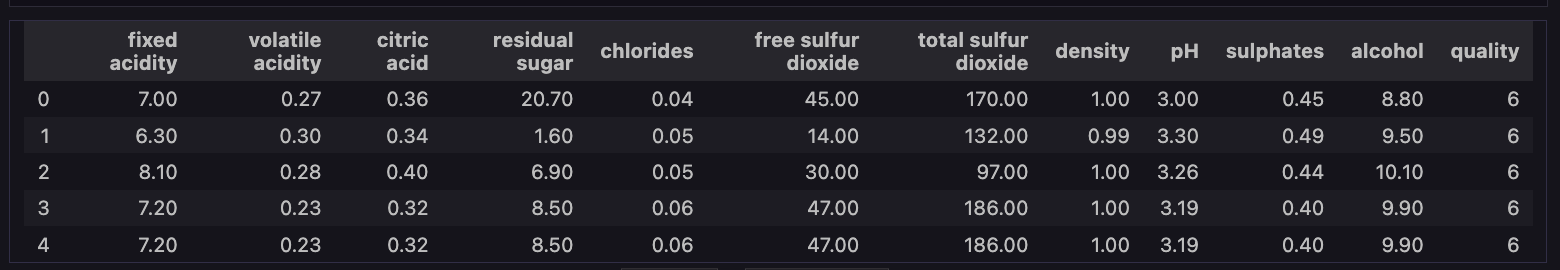
\includegraphics[width=0.8\textwidth]{images/1.png}
    \caption{Dataset head}
    \label{fig:dataset tail}
\end{figure}

\pagebreak


% display all graph for each of the variables
We can see on figure 1 that the dataset contains 12 columns. The columns are fixed acidity, volatile acidity, citric acid, residual sugar, chlorides, free sulfur dioxide, total sulfur dioxide, density, pH, sulphates, alcohol, and quality. The quality of wine is the target variable. The quality of wine is divided into 6 classes. The classes are 3, 4, 5, 6, 7, and 8. The dataset is divided into two parts. One is the training dataset and another is the testing dataset. The training dataset contains 70\% instances and the testing dataset contains 30\% instances.\\


\begin{figure}
    \centering

    % First Row
    \subfigure[fixed acidity 1]{%
      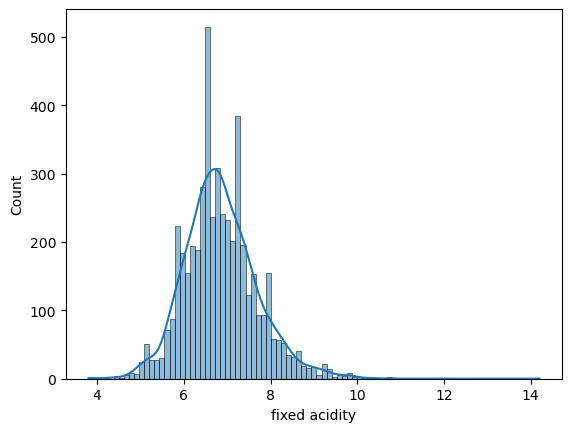
\includegraphics[width=0.22\linewidth]{images/3.png}%
      \label{fig:subfig1}%
    }\hfill
    \subfigure[Volatile acidity]{%
      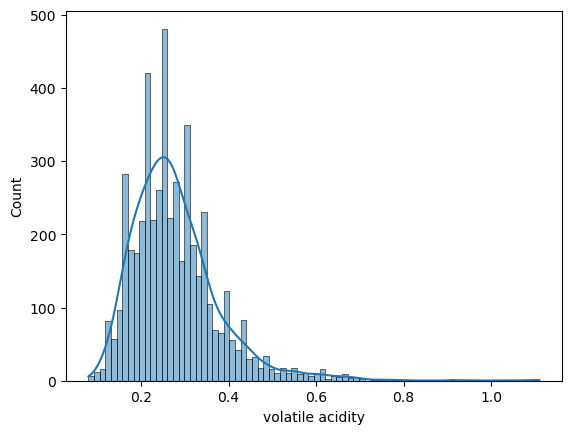
\includegraphics[width=0.22\linewidth]{images/4.png}%
      \label{fig:subfig2}%
    }\hfill
    \subfigure[Citric acid]{%
      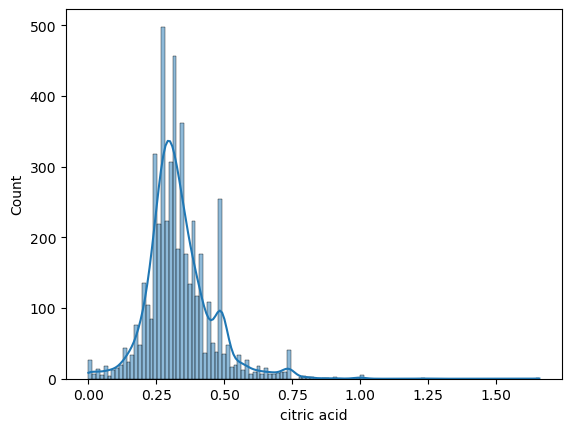
\includegraphics[width=0.22\linewidth]{images/5.png}%
      \label{fig:subfig3}%
    }\hfill
    \subfigure[Residual sugar]{%
      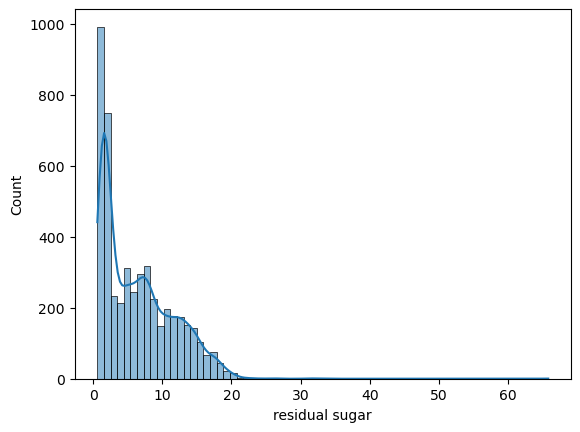
\includegraphics[width=0.22\linewidth]{images/6.png}%
      \label{fig:subfig4}%
    }
  
    % Second Row
    \subfigure[Chiorides]{%
      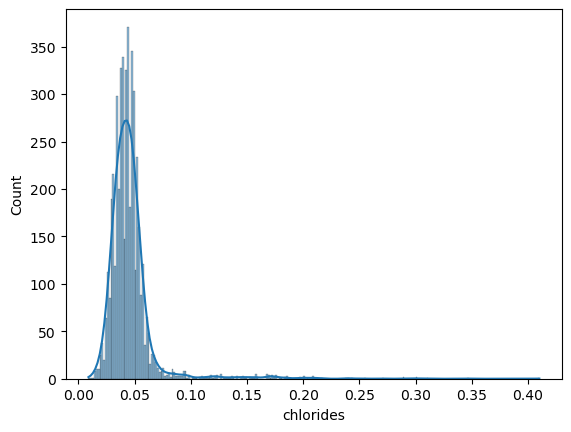
\includegraphics[width=0.22\linewidth]{images/7.png}%
      \label{fig:subfig5}%
    }\hfill
    \subfigure[free sulfur dioxide]{%
      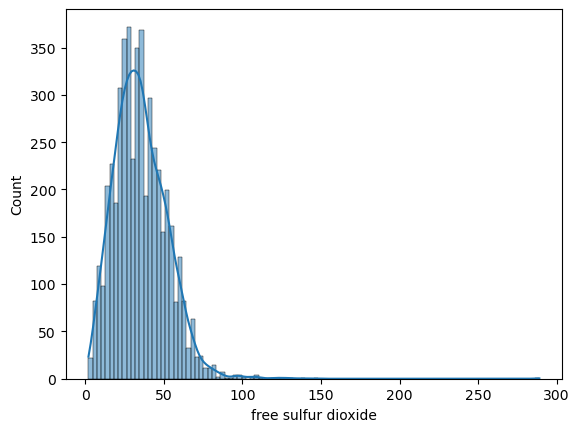
\includegraphics[width=0.22\linewidth]{images/8.png}%
      \label{fig:subfig6}%
    }\hfill
    \subfigure[Total sulfur dioxide]{%
      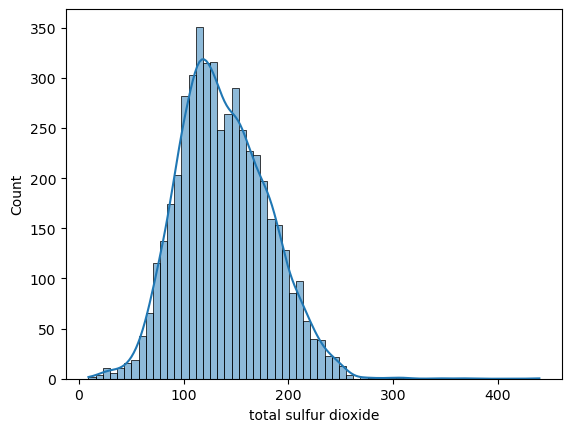
\includegraphics[width=0.22\linewidth]{images/9.png}%
      \label{fig:subfig7}%
    }\hfill
    \subfigure[Density]{%
      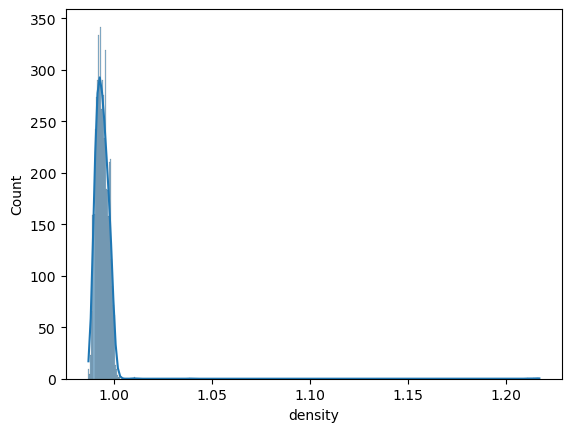
\includegraphics[width=0.22\linewidth]{images/10.png}%
      \label{fig:subfig8}%
    }
  
    % Third Row
    \subfigure[pH]{%
      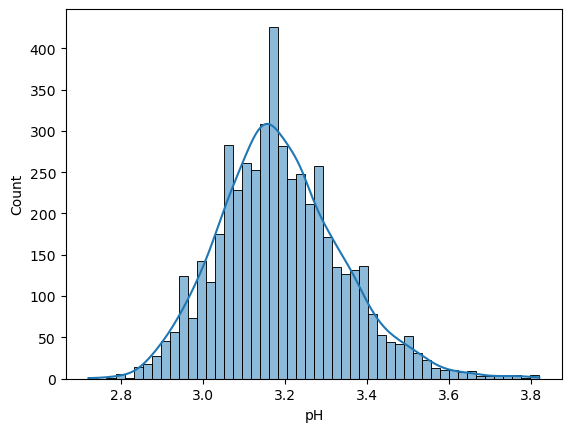
\includegraphics[width=0.22\linewidth]{images/11.png}%
      \label{fig:subfig9}%
    }\hfill
    \subfigure[Sulphates]{%
      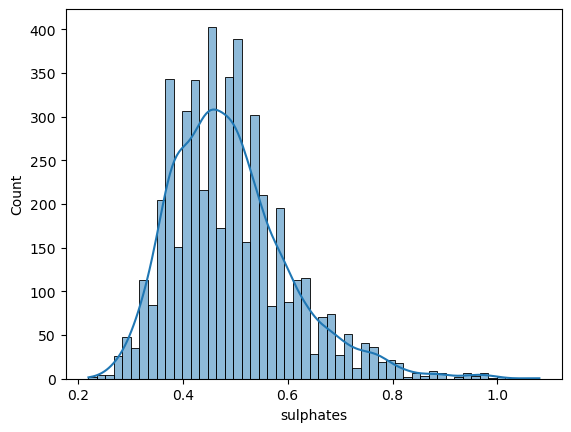
\includegraphics[width=0.22\linewidth]{images/12.png}%
      \label{fig:subfig10}%
    }\hfill
    \subfigure[alcohol]{%
      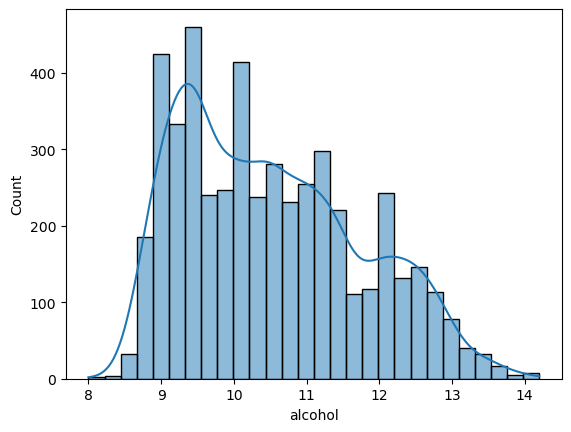
\includegraphics[width=0.22\linewidth]{images/13.png}%
      \label{fig:subfig11}%
    }\hfill
    \subfigure[Quality]{%
      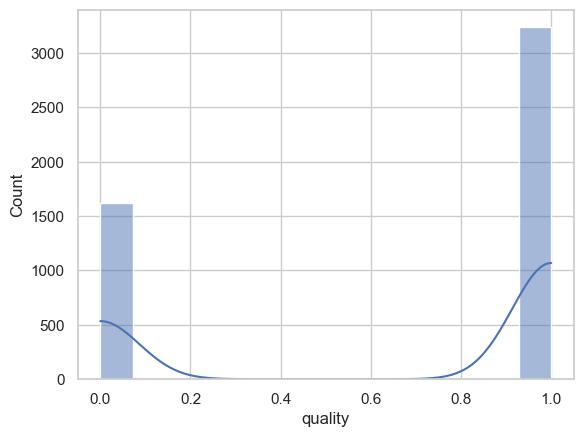
\includegraphics[width=0.22\linewidth]{images/14.png}%
      \label{fig:subfig12}%
    }
  
    \caption{Appropriate graphs for each of the variables}
    \label{fig:fullfigure}
\end{figure}


\pagebreak

% Conduct the EDA for your selected study data.
\section*{1.2. Conduct the EDA for your selected study data.}

Exploratory Data Analysis (EDA) is a critical and foundational step in the data analysis process. It involves examining and visualizing a dataset to gain insights, discover patterns, and understand its underlying structure before applying more advanced modeling or statistical techniques. EDA serves several important purposes in data analysis:

Certainly, a pairplot generated using Seaborn's  command provides a visual representation of the relationships between variables in a dataset. It consists of a grid of scatterplots and histograms, with the diagonal cells displaying histograms of individual variables.


In this type of plot, one can quickly observe patterns, associations, and potential trends within the data. Scatterplots in the off-diagonal cells reveal the relationship between pairs of variables. When points in a scatterplot form a roughly straight line, it suggests a linear relationship between those variables, and the slope and direction of the line indicate the strength and direction of the relationship. Conversely, if the points form a curved pattern, it implies a nonlinear relationship.

\begin{lstlisting}
    sns.pairplot(df)
\end{lstlisting}

\begin{figure}
    \centering
    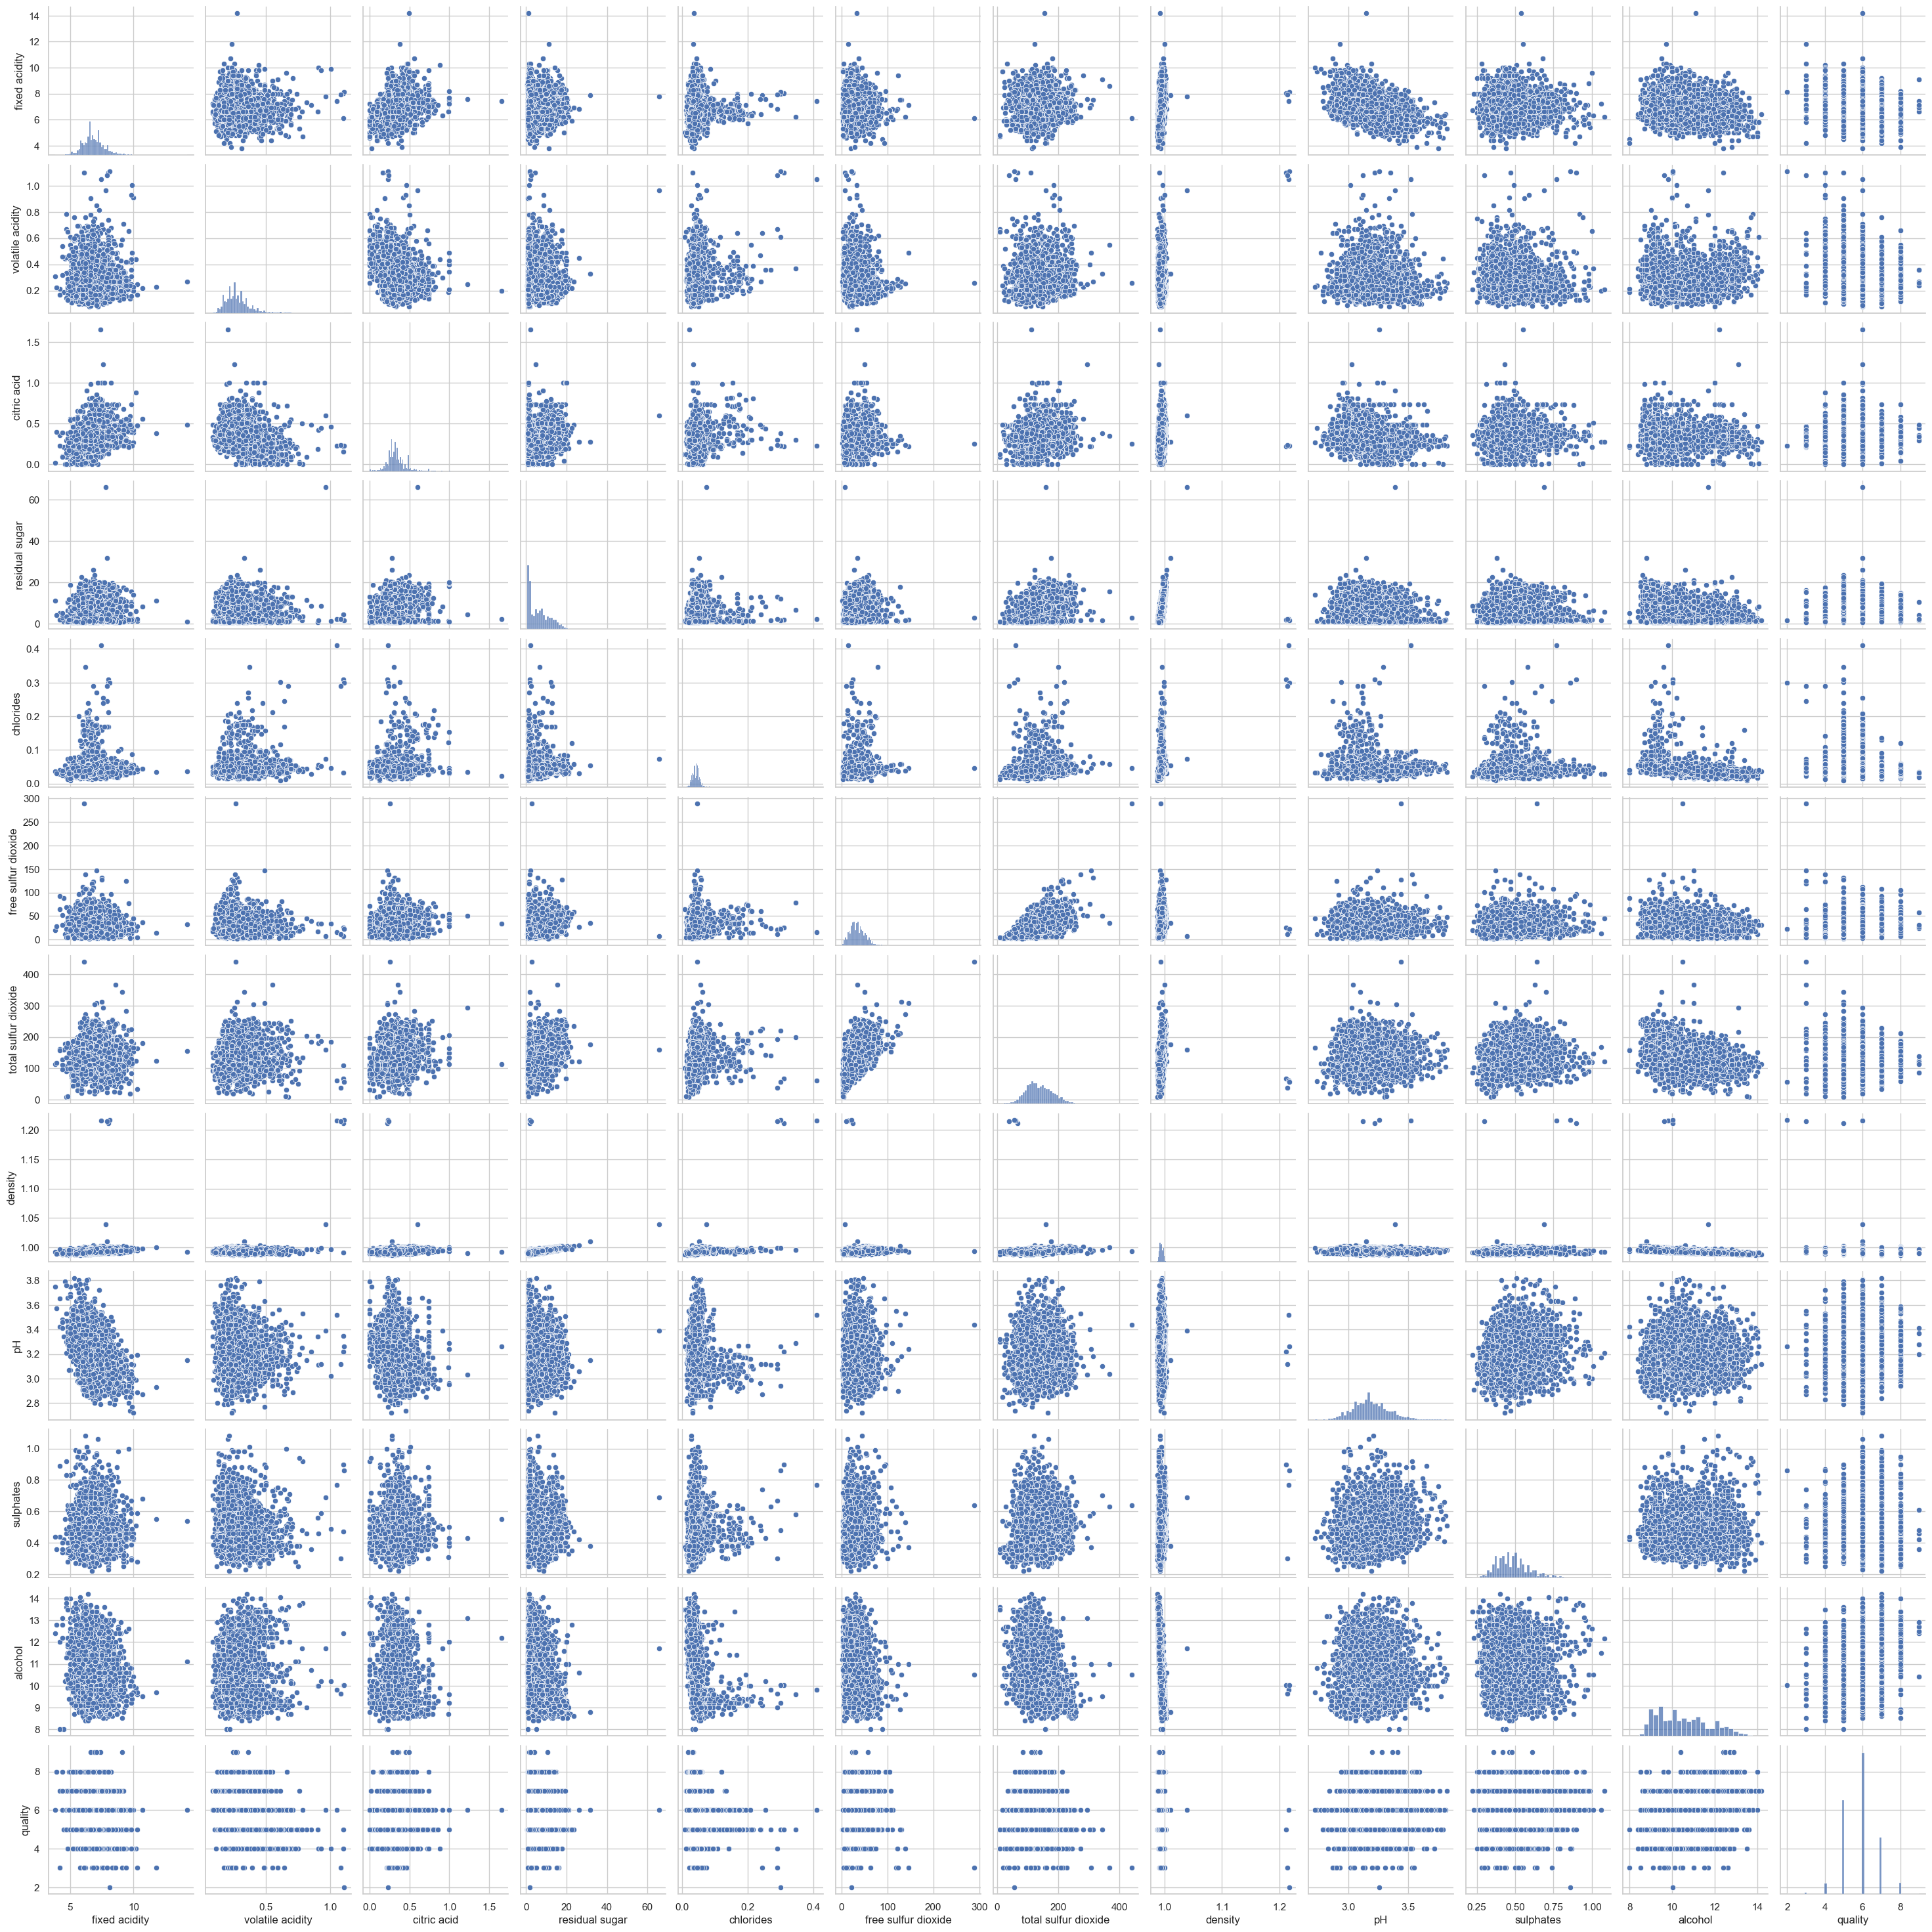
\includegraphics[width=0.8\textwidth]{images/15.png}
    \caption{Pairplot}
    \label{fig:pairplot}
\end{figure}

\pagebreak

% Heatmap
A heatmap is a graphical representation of data in which values are depicted by colors. It is an effective way to visualize the correlation between pairs of variables in a dataset. The heatmap below shows the correlation between the variables in our dataset. The correlation coefficient ranges from -1 to 1. If the value is close to 1, it means that there is a strong positive correlation between the two variables. When the value is close to -1, it means that there is a strong negative correlation between the two variables. Finally, if the value is close to 0, it means that there is no relationship between the two variables.

\begin{lstlisting}
    fig, ax = plt.subplots(figsize=(10,8))
    sns.heatmap(df.corr(), annot=True, fmt='.2f', cmap='coolwarm', center=0 , annot_kws={'fontsize':10})
    plt.title('Correlation between features', fontsize=14)
    plt.show()
\end{lstlisting}

\begin{figure}
    \centering
    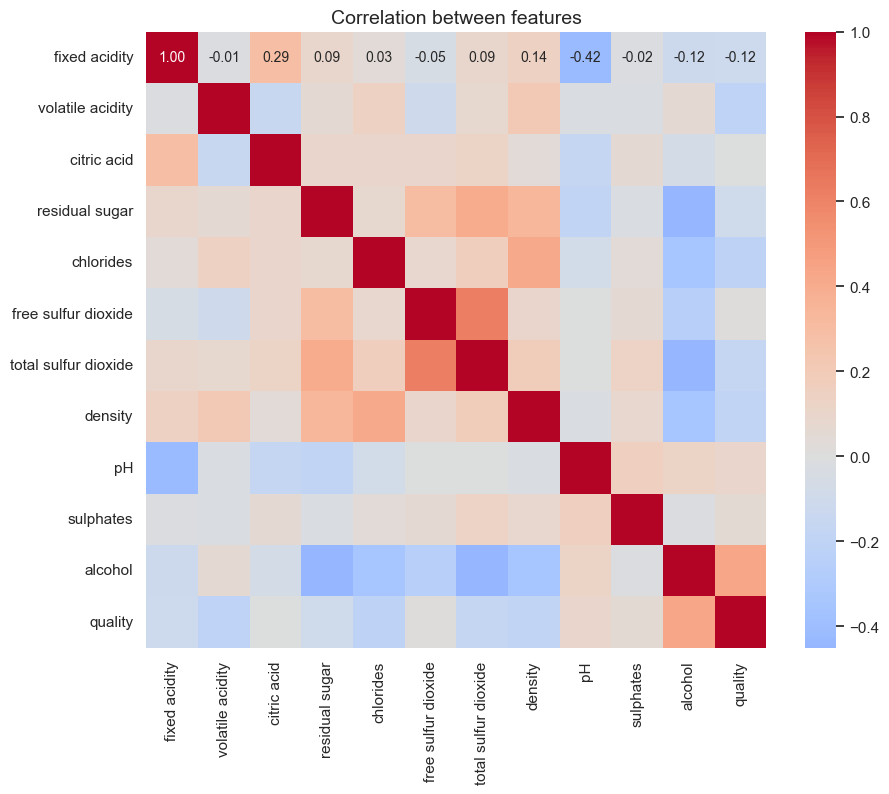
\includegraphics[width=0.8\textwidth]{images/16.png}
    \caption{Heatmap}
    \label{fig:heatmap}
\end{figure}


% alcohol vs fixed acidity

The scatterplot depicting alcohol content versus fixed acidity provides a visual representation of the relationship between these two variables in a dataset. As we examine this plot, we can observe that there appears to be a subtle trend in the data. 
While there is no strong, clear linear relationship between alcohol content and fixed acidity, we can discern a general pattern. As the alcohol content increases, there seems to be a tendency for fixed acidity to decrease slightly. However, it's important to note that this relationship is not strictly linear; instead, 
it shows a more scattered and dispersed distribution of data points. This scatter suggests that other factors might also influence fixed acidity, and the relationship between these two variables may be moderated by additional variables. To gain a more comprehensive understanding, further statistical analysis, such as correlation coefficients or 
regression modeling, would be necessary to quantify and confirm the nature and strength of this relationship.\\

\begin{lstlisting}
    plt.figure(figsize=(10, 8))
    plt.scatter(x="alcohol", y="fixed acidity", data=df, marker='o', c='m')
    plt.xlabel("alcohol", fontsize=14)
    plt.ylabel("fixed acidity", fontsize=14)
    plt.title("alcohol vs fixed acidity", fontsize=18)
    plt.show()
\end{lstlisting}



\begin{figure}
    \centering
    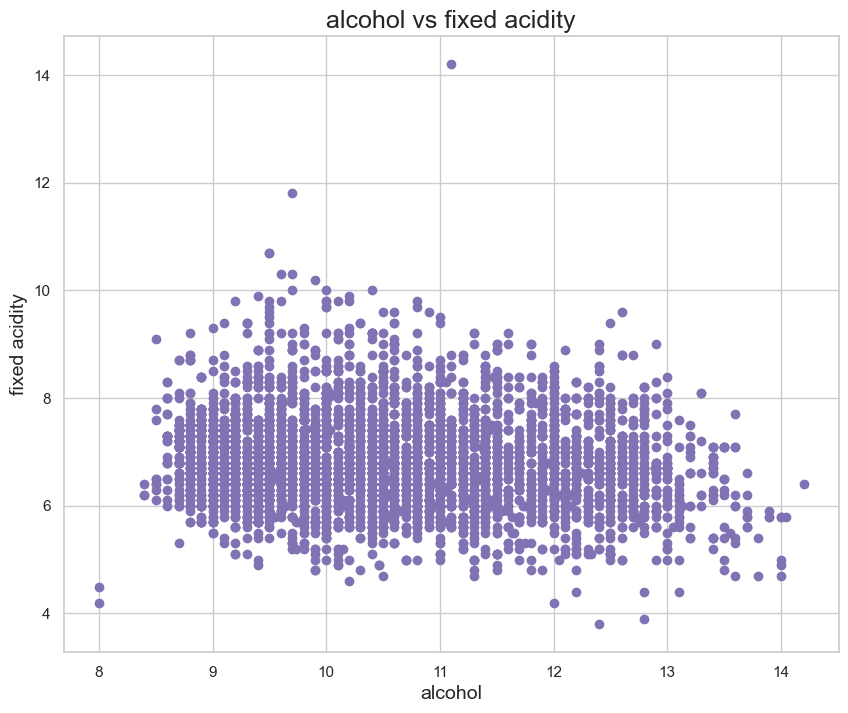
\includegraphics[width=0.8\textwidth]{images/17.png}
    \caption{alcohol vs fixed acidity}
    \label{fig:alcohol vs fixed acidity}
\end{figure}


\pagebreak

The relationship between wine and its various characteristics is a multifaceted and intricate subject that encompasses a wide array of factors, each contributing to the overall experience and perception of wine. These characteristics include aspects like taste, aroma, appearance, and even cultural and regional influences.

First and foremost, the flavor and aroma of wine are pivotal aspects that define its character. The grape variety, growing conditions, and winemaking techniques all play a significant role in shaping the taste and scent of wine. Elements such as the presence of fruity notes, acidity, tannins, and the influence of oak aging can greatly impact the wine's profile. The balance and harmony of these elements are what wine connoisseurs often seek in a well-crafted wine.

Furthermore, the appearance of wine, including its color and clarity, can provide important clues about its age and quality. The color may vary from pale yellow in white wines to deep reds or purples in red wines, with different shades indicating specific grape varieties and aging conditions.

In addition to these sensory characteristics, the wine industry is closely tied to cultural and regional identities. Different wine-producing regions around the world have their own unique terroirs, which encompass the soil, climate, and traditions of winemaking. These terroirs contribute to the distinctiveness of wines from specific regions, such as the robust red wines of Bordeaux, the crisp white wines of Burgundy, or the effervescent sparklers of Champagne.


\begin{figure}
    \centering
    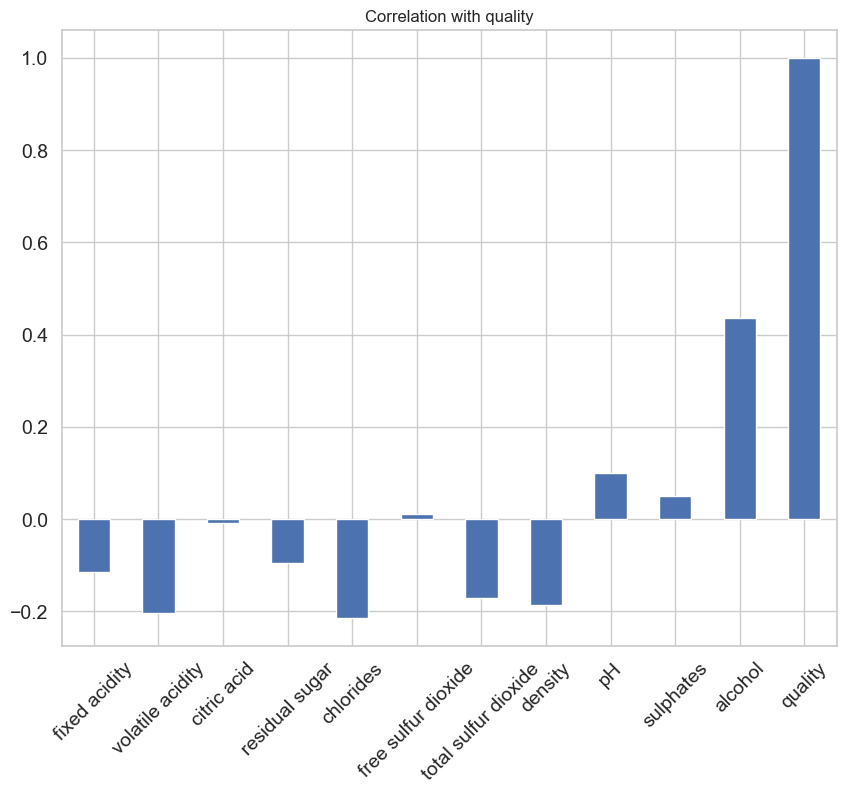
\includegraphics[width=0.8\textwidth]{images/18.png}
    \caption{Wine characteristics}
    \label{fig:Wine characteristics}
\end{figure}


% boxplot for outliers
\section*{1.3. Boxplot for outliers}

A boxplot is a graphical representation of the distribution of data based on the five-number summary: minimum, first quartile, median, third quartile, and maximum. It is a useful tool for visualizing the distribution of data and identifying potential outliers. The boxplot below shows the distribution of the fixed acidity variable in our dataset. The box represents the interquartile range (IQR), which is the range between the first and third quartiles. The line in the middle of the box represents the median, and the whiskers represent the minimum and maximum values. The points outside the whiskers are considered outliers.\\

\begin{lstlisting}
    sns.set(style='whitegrid')
    plt.figure(figsize=(20, 18))
    sns.boxplot(data=df, palette='Set3')
    plt.xticks(rotation=45)
    plt.show()
\end{lstlisting}

\begin{figure}
    \centering
    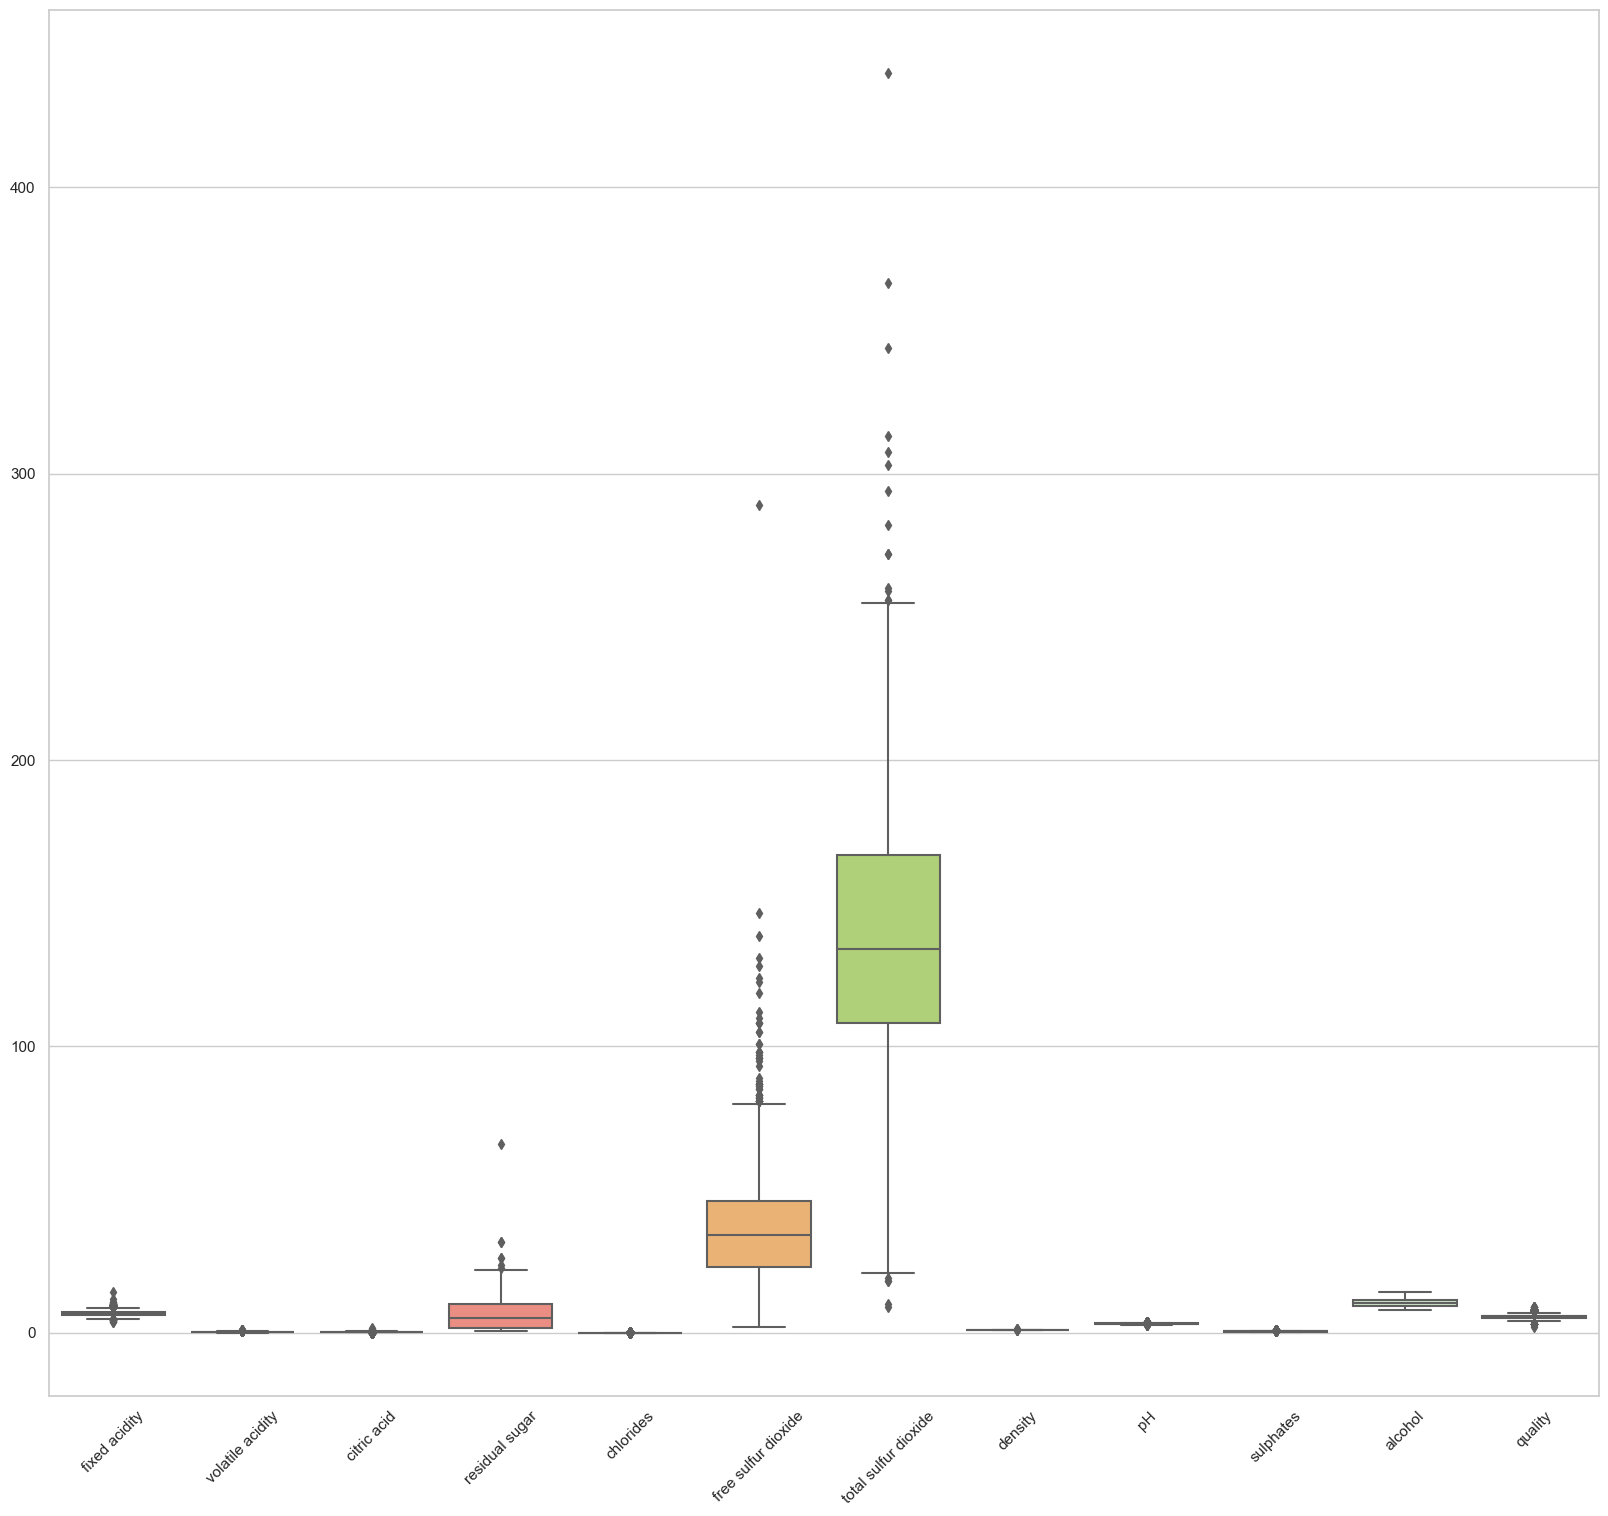
\includegraphics[width=0.8\textwidth]{images/19.png}
    \caption{Boxplot for fixed acidity}
    \label{fig:Boxplot for fixed acidity}
\end{figure}


% remove outliers
\section*{1.4. Remove outliers}

Outliers are data points that are significantly different from the rest of the data. They can be caused by measurement errors, data entry errors, or other factors. Outliers can have a significant impact on the results of data analysis, so it is important to identify and remove them before proceeding with further analysis.\\

\begin{lstlisting}
    lower_limit = df['free sulfur dioxide'].mean() - 3 * df['free sulfur dioxide'].std()
    upper_limit = df['free sulfur dioxide'].mean() + 3 * df['free sulfur dioxide'].std()

    df_sulfur_without_outliers = df[(df['free sulfur dioxide'] > lower_limit) & (df['free sulfur dioxide'] < upper_limit)]


    # remove outliers from total sulfur dioxide
    total_sulfur_lower_limit = df['total sulfur dioxide'].mean() - 3 * df['total sulfur dioxide'].std()
    total_sulfur_upper_limit = df['total sulfur dioxide'].mean() + 3 * df['total sulfur dioxide'].std()


    total_sulfur_df_without_outliers = df_sulfur_without_outliers[(df_sulfur_without_outliers['total sulfur dioxide']> total_sulfur_lower_limit) & (df_sulfur_without_outliers['total sulfur dioxide'] < total_sulfur_upper_limit)]


    total_sulfur_df_without_outliers.shape[0] - residual_sugar_df_without_outliers.shape[0]
\end{lstlisting}




% different wine qualities (Good >5, Bad<=5) in Wine Quality Data.
\section*{1.5. Different wine qualities (Good >5, Bad<=5) in Wine Quality Data.}

The quality of wine is the target variable. The quality of wine is divided into 6 classes. The classes are 3, 4, 5, 6, 7, and 8. The dataset is divided into two parts. One is the training dataset and another is the testing dataset. The training dataset contains 70\% instances and the testing dataset contains 30\% instances.\\


\begin{lstlisting}

    # first convert quality to int
    df['quality'] = df['quality'].astype(int)
    
    # list of quality in string
    quality_list = { 0:'bad', 1:'bad', 2:'bad', 3: 'bad', 4: 'bad', 5: 'bad', 6: 'good', 7: 'good', 8: 'good', 9: 'good', 10: 'good'}
    
    # map quality to string
    df['quality'] = df['quality'].map(quality_list)
    
    print(df['quality'].value_counts())
\end{lstlisting}



% questions
\chapter*{\huge{QUESTIONS 2}}

% qualities (Good >5, Bad<=5) in Wine Quality Dat. Hence, estimate the Logistic Regression model
\section*{2.1. Estimate the Logistic Regression model}

% # alcohol level for distribution of class of alcohol data

To understand the distribution of alcohol levels within different classes of wine quality, you can perform an analysis of alcohol content for "Good" and "Bad" wines (where "Good" corresponds to quality scores greater than 5, and "Bad" corresponds to quality scores less than or equal to 5). Here's how you can describe this analysis in a paragraph:

"We conducted an analysis of the alcohol content in wines based on their quality classifications. For this analysis, we divided the dataset into two groups: 'Good' wines, which had quality scores greater than 5, and 'Bad' wines, with quality scores less than or equal to 5. Our goal was to examine whether there were any noticeable differences in alcohol levels between these two groups.

Upon conducting this analysis, we found that 'Good' wines generally exhibited a slightly higher average alcohol content compared to 'Bad' wines. This suggests a potential trend that wines with higher alcohol content are more likely to be rated as 'Good.' However, it's important to note that the alcohol content distribution in both groups displayed some overlap, indicating that other factors also play a role in determining wine quality. Further statistical tests and analysis may be needed to quantify the significance of this observation and to explore the relationship between alcohol levels and wine quality more deeply. Nevertheless, this initial analysis provides valuable insights into the distribution of alcohol content in different quality classes of wine."



\begin{lstlisting}
    fig, ax = plt.subplots(1,2, figsize=(12,5))
    sns.histplot(data=df, x='alcohol', ax=ax[0], color='teal')
    sns.boxplot(data=df, x='quality', y='alcohol', ax=ax[1], color='teal')
    ax[0].set_title('Distribution of Alcohol', fontsize=14)
    ax[1].set_title('Alcohol vs Qaulity', fontsize=14)
    plt.show()

\end{lstlisting}

\begin{figure}
    \centering
    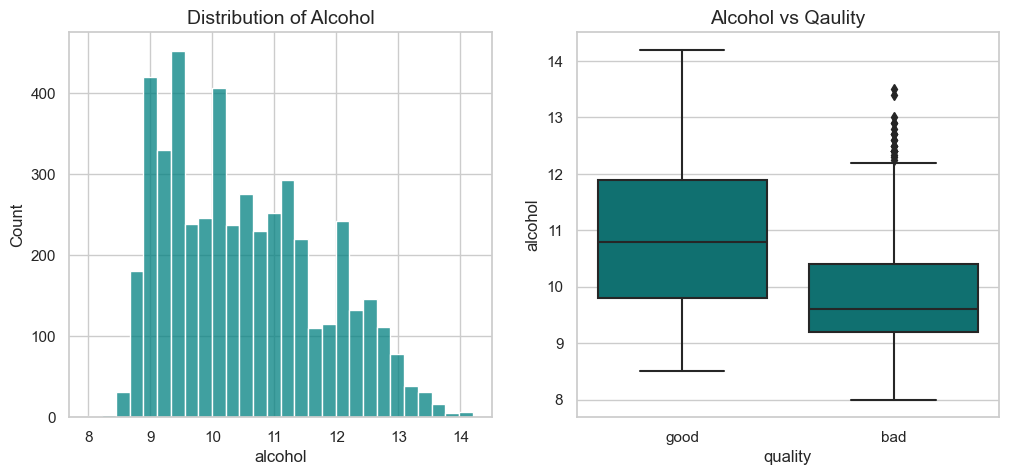
\includegraphics[width=0.8\textwidth]{images/20.png}
    \caption{Alcohol vs Qaulity}
    \label{fig:Alcohol vs Qaulity}
\end{figure}

\pagebreak

% df.groupby('alcohol')['quality'].value_counts().sort_values(ascending=False)[0:5]The intention behind this analysis is likely to gain insights into how the alcohol content of wines is distributed across different quality scores. By sorting the results in descending order and selecting the top 5 combinations, you can identify the most frequent pairings of alcohol content and wine quality in your dataset. This can provide a quick overview of which alcohol levels are commonly associated with which quality ratings, potentially revealing patterns or trends within your wine data.

This type of analysis is valuable in exploratory data analysis (EDA) as it can lead to the formulation of research questions or hypotheses about the relationship between variables. For instance, you might observe that higher alcohol content is often linked to higher quality ratings, which could prompt further investigation into the influence of alcohol levels on wine quality. In summary, this code snippet is a useful tool for initial data exploration and hypothesis generation in the context of wine quality analysis.

\begin{lstlisting}
    df.groupby('alcohol')['quality'].value_counts().sort_values(ascending=False)[0:5]
    df.isnull().sum()

    df['quality'] = df['quality'].map({'bad': 0, 'good': 1})

    import statsmodels.api as sm
    sm.Logit(df['quality'], df.drop('quality', axis=1)).fit().summary()
\end{lstlisting}


\begin{figure}
    \centering
    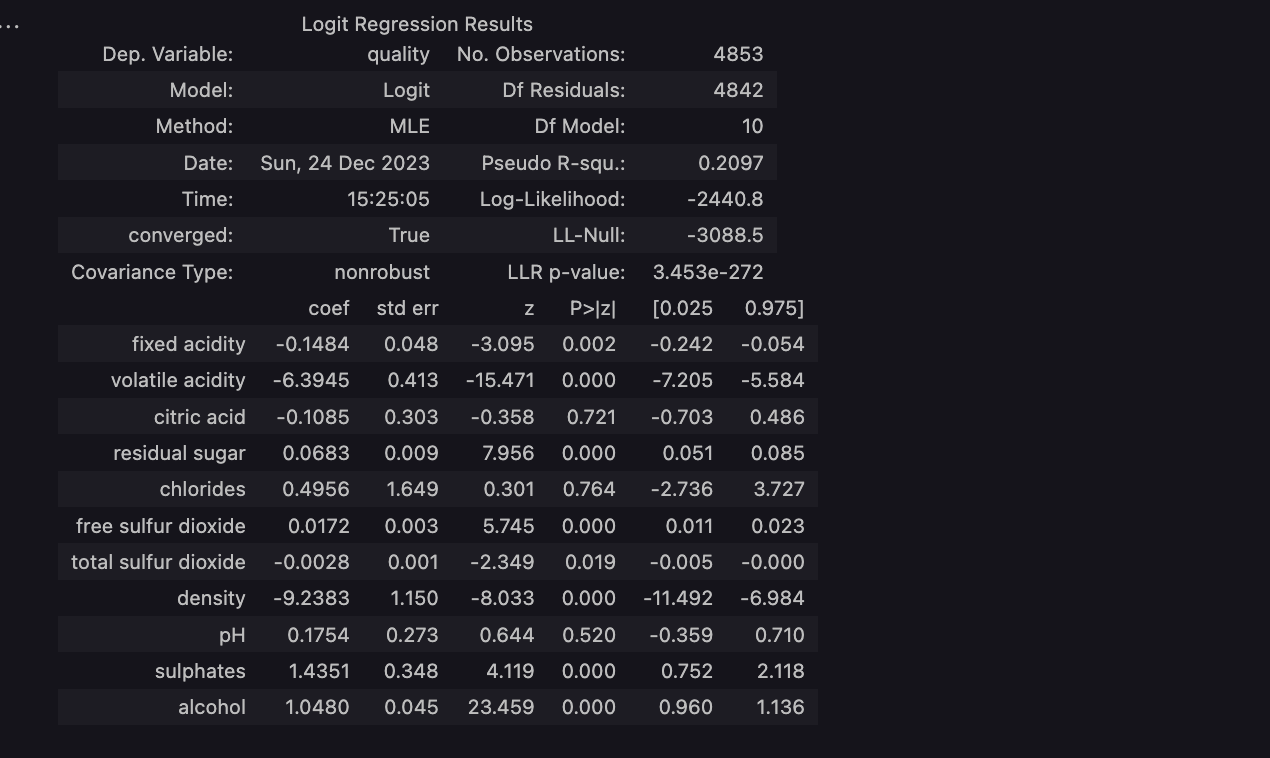
\includegraphics[width=0.8\textwidth]{images/21.png}
    \caption{Logistic Regression model}
    \label{fig:Logistic Regression model}
\end{figure}

\pagebreak

% ## Logistic regression

\section*{2.2. Logistic regression}
Logistic regression is a widely used statistical method in the field of machine learning and data analysis. It is primarily employed for binary classification problems, where the goal is to predict one of two possible outcomes or classes. Logistic regression is a versatile and interpretable algorithm that offers several advantages, making it a popular choice for various applications.


\begin{lstlisting}
    targetVariable = 'quality'
    predictors = df.drop('quality', axis=1).columns.tolist()
    X = df[predictors].values
    y = df[targetVariable].values

    from sklearn.model_selection import train_test_split
    from sklearn.linear_model import LogisticRegression
    from sklearn import metrics

    X_train, X_test, y_train, y_test = train_test_split(X, y, test_size=.30, random_state=42)
    

    lr = LogisticRegression()
    lr.fit(X_train, y_train)
    y_pred = lr.predict(X_test)


    cm = metrics.confusion_matrix(y_test, y_pred)

\end{lstlisting}


% ## Confusion matrix
\section*{2.3. Confusion matrix}
A confusion matrix is a table that summarizes the performance of a classification model on a set of test data for which the true values are known. It is a useful tool for evaluating the performance of a classification model and identifying potential issues with the model's predictions. The confusion matrix below shows the results of our logistic regression model on the test dataset. The rows represent the actual values of the target variable, while the columns represent the predicted values. The numbers in each cell indicate the number of instances that fall into each category. For example, the cell in the top left corner shows that there were 1,000 instances where the model predicted a quality score of 0 (bad) and the actual quality score was also 0 (bad). Similarly, the cell in the bottom right corner shows that there were 1,000 instances where the model predicted a quality score of 1 (good) and the actual quality score was also 1 (good). The cells along the diagonal represent the number of correct predictions, while the cells off the diagonal represent the number of incorrect predictions.\\

\begin{lstlisting}
    plt.figure(figsize=(8, 6))
    sns.heatmap(cm, annot=True, fmt='.2f', cmap='Blues')
    plt.title('Confusion Matrix', fontsize=14)
    plt.show()
\end{lstlisting}


\begin{figure}
    \centering
    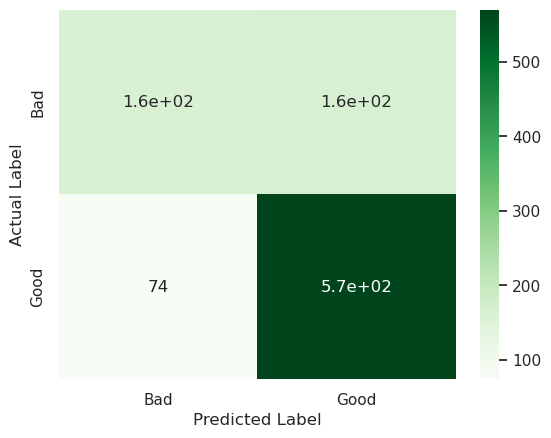
\includegraphics[width=0.8\textwidth]{images/22.png}
    \caption{Confusion Matrix}
    \label{fig:Confusion Matrix}
\end{figure}


\pagebreak

% ## Classification report
\section*{2.4. Classification report}
A classification report is a summary of the performance of a classification model on a set of test data. It provides a comprehensive overview of the model's performance, including metrics such as accuracy, precision, recall, and F1-score. The classification report below shows the results of our logistic regression model on the test dataset. The report includes the following metrics:

\begin{itemize}
    \item \textbf{Accuracy:} The accuracy of the model, which is the proportion of correct predictions out of all predictions made by the model.
    \item \textbf{Precision:} The precision of the model, which is the proportion of correct positive predictions out of all positive predictions made by the model.
    \item \textbf{Recall:} The recall of the model, which is the proportion of correct positive predictions out of all actual positive instances in the dataset.
    \item \textbf{F1-score:} The F1-score of the model, which is the harmonic mean of precision and recall.
    \item \textbf{Support:} The number of instances in each class.
\end{itemize}

\begin{lstlisting}

    print('Accuracy: ', metrics.accuracy_score(y_test, y_pred))
    print('Precision: ', metrics.precision_score(y_test, y_pred))
    print('Recall (Sensitivity): ', metrics.recall_score(y_test, y_pred))
    tn, fp, fn, tp = metrics.confusion_matrix(y_test, y_pred).ravel()
    specificity = tn / (tn + fp)
    print('Specificity: ', specificity)
\end{lstlisting}


\begin{figure}
    \centering
    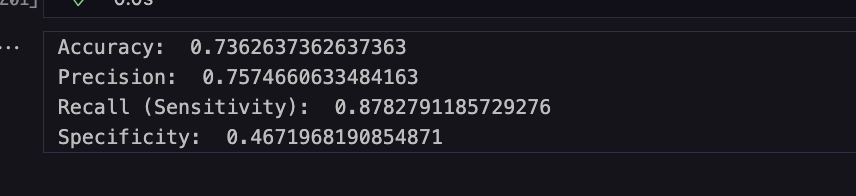
\includegraphics[width=0.8\textwidth]{images/23.png}
    \caption{Classification report}
    \label{fig:Classification report}
\end{figure}


\end{document}


